\chapter{Confidence intervals for prevalence estimates from complex surveys with imperfect assays}
\label{ch:content_1}
\graphicspath{{figures/ch_3/}}

\section{Introduction}

Estimating and quantifying uncertainty for disease prevalence is a standard task in epidemiology.
For rare events, these estimates are highly sensitive to misclassification \citep{hemenwaySelfDefense}, making adjustments for sensitivity and specificity critically important.
While estimating prevalence (or any event proportion in a population) in complex surveys and adjusting estimates for misclassification have been well studied separately, performing both of these tasks simultaneously remains relatively unexplored. This paper fills that gap by studying estimates and confidence intervals for prevalence from complex surveys with misclassification.
We develop a new tractable confidence interval procedure designed to guarantee coverage.
Our confidence interval combines three statistical methods: (1) the gamma confidence interval for directly standardized rates is applied to the apparent prevalence \citep{FayF:1997}
and (2) standard misclassification adjustments to that apparent prevalence for sensitivity and specificity \citep{Roga:1978} are used together with (3) the melding method, which allows combination of confidence intervals for different parameters \citep{FayP:2015}.
We show by simulation only (there are no proofs of guaranteed coverage) that, with a complex survey with low prevalence and misclassification, our method appears to have at least nominal coverage.
Even in special cases (e.g., simple random samples with imperfect assays, or weighted samples with perfect assays) where there are existing methods, our new method has at least nominal simulated coverage. while some of the tractable existing methods may under-cover.
The cost for apparently achieving nominal coverage is that our intervals may be quite wide in some situations.


Recent overviews of confidence interval procedures for prevalence in surveys without misclassification are provided by \citet{Dean:2015} and \citet{franco2019}.
For simple random sample surveys with imperfect sensitivity and specificity, \citet{Lang:2014} proposed an approximate confidence interval that performed well in simulations.
Recent works by \citet{DiCi:2021} and \citet{Cai:2020} study both valid (i.e., exact) and approximate intervals.
Their valid intervals use test inversion and the adjustment of \citep{Berg:1994}, while their approximation intervals use the bootstrap with the test inversion approach.
Fewer methods are available for constructing frequentist confidence intervals for prevalence estimates from complex surveys while adjusting for sensitivity and specificity.
\citet{Kali:2021} developed one such method that is closely related to one of the methods presented here, but that method's properties were not studied.
\citet{Cai:2020} (see also discussion in \citep{DiCi:2021}) modify their approximation approach to allow sample weights for strata or individual specific weights.
Another recent advancement is the method developed by \citet{rosin2021estimating} that makes use of asymptotic normal approximations, which reduce to the Wald interval when sensitivity and specificity are perfect.
This problem has also previously been addressed in Bayesian literature, recently by \citet{GelmanBayes}.

We work up to our ultimate goal in stages.
First, in Section~\ref{ch_3:sec:srs-imperfect}, we propose confidence intervals for simple random samples where prevalence is assessed with an assay with imperfect sensitivity and/or specificity.
Next, in Section~\ref{ch_3:sec:weight-perfect}, we present confidence intervals for weighted samples where prevalence is assessed with an assay without misclassification.
In Section~\ref{ch_3:sec:weight-imperfect}, we combine these methods to create confidence intervals for weighted samples where prevalence is assessed with an assay with imperfect sensitivity and specificity.
Because the combined method reduces to one of the first two methods as a special case, we can think of the first two stages as testing the combined method in those cases.
Finally, in Section~\ref{ch_3:sec:complex-surveys} we show how certain complex surveys may fit into the format for our new method.

In simulations, we compare our method to established frequentist competitors and show through simulations that it beats the best of those in each of the three stages with respect to guaranteeing coverage.
However, in some simulated settings, our proposed methods are overly conservative, meaning that they demonstrate higher than nominal coverage, while competitor methods maintain closer to nominal coverage.
We did not include in our simulations some recent methods that have been developed in response to the COVID-19 pandemic \citep{Cai:2020,DiCi:2021,rosin2021estimating}.
The exact method of \citep{DiCi:2021} would guarantee coverage, although applying it to a survey with a large number of strata would be ``computationally expensive,'' and it has not been applied to surveys using post-stratification weighting. In contrast, our new method can very tractable in those situations.


\section{Confidence Interval Methods}

\subsection{Notation and Problem Set-up}
\label{ch_3:sec-notation}


To introduce notation, consider first the stratified simple random sample.
Suppose we have a population partitioned into \( K \) strata, with \( N_1, N_2, \ldots, N_K \) individuals in the \( K \) strata of the population.
We sample \( n_1, n_2, \ldots, n_K \) individuals via a simple random sample from each of the \( K \) strata to have an assay performed on each individual to determine who has the disease.
Let \( X_i \) be the number of positive results from an assay performed on the \( n_i \) individuals from stratum \( i \) and assume \( X_i \sim \operatorname{Binomial}(n_i, \theta_i) \), where \( \theta_i \) is the population frequency of positive results for assays performed on individuals from stratum \( i \).
Similarly, let \( X_i^* \) be the unobserved true number of people with the disease among the \( n_i \) individuals from stratum \( i \) and assume \( X_i^* \sim \operatorname{Binomial}(n_i, \theta_i^*) \), where \( \theta_i^* \) is the population frequency of cases in stratum \( i \).
In the case of a perfect assay, \( \theta_i = \theta_i^* \).




Therefore, the population prevalence is

\begin{equation}
    \beta^* = \frac{\sum_{i=1}^K N_i \theta_i^*}{\sum_{j=1}^K N_j} = \sum_{i=1}^K w_i \theta_i^*,
    \label{ch_3:eq:pop-prev}
\end{equation}

and the apparent prevalence is

\begin{equation}
    \beta = \frac{\sum_{i=1}^K N_i \theta_i}{\sum_{j=1}^K N_j} = \sum_{i=1}^K w_i \theta_i,
    \label{ch_3:eq:app-prev}
\end{equation}

where \( w_i = N_i / \sum_{j=1}^K N_j \) and, therefore, \( \sum_{i=1}^K w_i = 1 \).
This set-up will approximately work for other complex survey samples, where we can estimate survey weights such that the complex survey sample may be treated as a multinomial sample with probabilities proportional to those weights (see Section~\ref{ch_3:sec:complex-surveys}).

We can relate $\theta_i$ and $\theta_i^*$ using the sensitivity ($\phi_p$) and specificity (1-$\phi_n$) of the assay,
where $\phi_p$ and $\phi_n$ are the proportion of positive assays from a population of positive controls (i.e., individuals known to have the disease) and
negative controls (i.e., individuals known to be without the disease), respectively. Then
$\theta_i = \phi_p \theta_i^* + \phi_n (1-\theta_i^*)$, or equivalently \citep{Roga:1978},
\begin{eqnarray*}
\theta_i^* & = & \frac{ \theta_i - \phi_n }{\phi_p - \phi_n},
\end{eqnarray*}
and we have
\begin{align}
\begin{split}
  \beta^*   =&   \sum_{i=1}^K w_i \theta_i^*
            =  \sum_{i=1}^K w_i \left( \frac{\theta_i - \phi_n}{\phi_p - \phi_n} \right) \\
            =&   \frac{\sum_{i=1}^K w_i \theta_i}{\phi_p - \phi_n} - \frac{\phi_n \sum_{i=1}^K w_i}{\phi_p - \phi_n}
            =   \frac{\sum_{i=1}^K w_i \theta_i}{\phi_p - \phi_n} - \frac{\phi_n}{\phi_p - \phi_n}
            \label{ch_3:eq:long-beta}
\end{split}
\end{align}


Suppose the assay is measured on \( m_n \) individuals known not to have the disease and on \( m_p \) individuals known to have the disease.
Let \( C_n \) and \( C_p \) be the number who test positive from the respective samples.
Assume that the negative and positive controls act like simple random samples from their respective populations.
Thus, \( C_n \sim \operatorname{Binomial}(m_n, \phi_n) \) where \( 1 - \phi_n \) is the specificity of the assay, and \( C_p \sim \operatorname{Binomial}(m_p, \phi_p) \), where \( \phi_p \) is the sensitivity of the assay.
Let \( \hat{\theta}_i = \frac{X_i}{n_i} \), \( \hat{\phi}_n = \frac{C_n}{m_n} \), and \( \hat{\phi}_p = \frac{C_p}{m_p} \).
Then a plug-in estimator for \( \beta^* \) is
\begin{equation}
    \hat{\beta}^* = \frac{\sum_{i=1}^K w_i \hat{\theta}_i}{\hat{\phi}_p - \hat{\phi}_n} - \frac{\hat{\phi}_n}{\hat{\phi}_p - \hat{\phi}_n}. \label{ch_3:eq:betastarhat}
\end{equation}

This estimator serves as an important basis for developing confidence intervals in this work.
Section~\ref{ch_3:sec:srs-imperfect} is concerned with confidence intervals for \( \beta^* \) in the case where \( K = 1 \), \( \phi_n > 0 \), \( \phi_p < 1 \), i.e., estimating prevalence from a simple random sample with an imperfect assay.
Section~\ref{ch_3:sec:weight-perfect} is concerned with confidence intervals for \( \beta^* \) in the case where \( K > 1 \), \( \phi_n = 0 \), \( \phi_p = 1 \), i.e., estimating prevalence from a weighted sample with a perfect assay.
Section~\ref{ch_3:sec:weight-imperfect} is concerned with confidence intervals for \( \beta^* \) in the case where \( K > 1 \), \( \phi_n > 0 \), \( \phi_p < 1 \), i.e., estimating prevalence from a weighted sample with an imperfect assay.

\subsection{Estimating Prevalence from a Simple Random Sample with an Imperfect Assay}
\label{ch_3:sec:srs-imperfect}

First we consider the scenario where \( K = 1 \), \( \phi_n > 0 \), and \( \phi_p < 1 \).
We develop a confidence interval for the population prevalence, \( \beta^* \).
When \( K = 1 \), the estimand in Equation~\ref{ch_3:eq:long-beta} becomes $\beta^* = (\theta_1 - \phi_n)/(\phi_p-\phi_n)$. We have $\phi_p > \phi_n$ for any useful assay, and since the sample is a mixture of individuals with and without the disease of interest, $\phi_p \geq \theta_1 \geq \phi_n$. The estimator of $\beta^*$ is
%in Equation~\ref{ch_3:eq:betastarhat} becomes

\begin{equation}
\hat{\beta}^* \equiv
g(\hat{\theta}_1, \hat{\phi}_n, \hat{\phi}_p)
\equiv
\left\{
\begin{array}{ll}
1 & \mbox{ if $\hat{\phi}_n < \hat{\phi}_p \leq \hat{\theta}_1$ }  \\
\frac{\hat{\theta}_1 - \hat{\phi}_n}{\hat{\phi}_p - \hat{\phi}_n} &
\mbox{ if $\hat{\phi}_p > \hat{\theta}_1 \geq \hat{\phi}_n$ } \\
0 & \mbox{ otherwise.}
\end{array}
\right.
\label{ch_3:eq:srs-beta-est}
\end{equation}
% Damon, that definition is arbitrary, it is just used so that



To create a confidence interval for \( \hat{\beta}^* \), we use a generalization of the melding method \citep{FayP:2015}, which makes use of lower and upper confidence distributions on functions of independent estimators to account for variability in \( \hat{\theta}_1 \), \( \hat{\phi}_n \), and \( \hat{\phi}_p \).
Before describing the melding method, we briefly review confidence distributions.

Confidence distributions are frequentist estimators of a parameter, which can be used similarly to the bootstrap or posterior distributions.
For continuous responses (and asymptotically for discrete responses), one can formally define confidence distributions without relying on previously derived confidence interval procedures \citep{Xie2013}, but for intuition with discrete responses, it is easier to derive confidence distributions the classical way, i.e., directly from confidence interval procedures.
Here, we reproduce the definition of confidence distributions from Section~\ref{ch_2:sec:confidence_distributions}.
For discrete responses, there are two confidence distributions (the lower and upper ones), used to ensure validity of the resulting inferences.
Under the classical derivation, we can create random variables associated with the lower and upper confidence distributions from two one-sided, nested, confidence interval procedures, where for a nested confidence interval procedure, the $(1-\alpha_1)$ interval is a subset of the $(1-\alpha_2)$ interval whenever $(1-\alpha_1) \leq (1-\alpha_2)$.
Denote those one-sided intervals by $[L({\bf x},1-\alpha), \infty)$ and $(-\infty, U({\bf x},1-\alpha)]$, which are defined for any observed data ${\bf x}$, and $(1-\alpha) \in (0,1)$.
For fixed ${\bf x}$, define the lower and upper confidence distribution random variables as $L({\bf x}, A)$ and $U({\bf x},B)$, where $A$ and $B$ are independent uniform random variables.
Then a $100(1-\alpha)\%$ central confidence interval has the $(\alpha/2)$th quantile of $L({\bf x}, A)$ as the lower limit, and the $(1-\alpha/2)$th quantile of $U({\bf x},B)$ as the upper limit.

Because each estimated component in Equation~\ref{ch_3:eq:srs-beta-est} is a binomial probability parameter, we now focus on the confidence distributions associated with the exact binomial confidence interval.
For a binomial experiment with \( x \) successes out of \( n \) trials, the lower confidence distribution is \( \operatorname{Beta}(x, n - x + 1) \) with associated random variable \( B^L \), and the upper confidence distribution is \( \operatorname{Beta}(x + 1, n - x)\) with random variable \( B^U \), where for $a>0$ we let \( \operatorname{Beta}(0,a) \) and \( \operatorname{Beta}(a,0) \) be point masses at 0 and 1, respectively.
This result comes from the relationship between the binomial and beta distributions, namely $\mathrm{Pr}[X \leq x] = \mathrm{Pr}[B > \theta]$, where $B \sim \operatorname{Beta}(x + 1, n - x)$ for $x \in \left\{ -1,0, 1, \ldots, n \right\}$ (see e.g., \citep[Section~2]{Blyth1986}, \citep[Section~S2]{Fay2021}).
Additionally, in the binomial case, the lower and upper confidence distributions are equivalent to
the posterior distributions that result from using well-calibrated null preference priors \citep{Fay2021}.
Let \( q(a, W) \) be the \( a \)th quantile of a random variable \( W \). Then the exact \( 1 - \alpha \)\% central confidence interval of \citep{10.1093/biomet/26.4.404} for the binomial parameter is
\begin{equation}
\left\{ q \left( \frac{\alpha}{2}, B^L \right), q \left( 1 - \frac{\alpha}{2}, B^U, \right) \right\}.
\label{ch_3:eq:C-P}
\end{equation}

\citet{FayP:2015} proposed the melding method for obtaining confidence intervals for functions of two parameters that are monotonic within the allowable range for each parameter, given the other is fixed.
The melding method uses quantiles of those functions except replacing lower or upper confidence distribution random variables for their associated parameter in the function.
Here, we generalize that method to $\beta^*$, which is a function of three parameters.
When $1 \geq \phi_p > \theta_1 > \phi_n \geq 0$ then $\beta^*$ is monotonically increasing in $\theta_1$, monotonically decreasing in $\phi_p$, and monotonically decreasing in $\phi_n$.
For an assessment of monotonicity in other scenarios, see Appendix~\ref{ch_3:sec:monotonicity}.
Then the \( 1-\alpha \)\% confidence interval for \( \beta^* \) is

\begin{equation}
    \left\{ q \left( \frac{\alpha}{2}, g \left\{ B_{\theta_1}^L, B_{\phi_n}^U, B_{\phi_p}^U \right\} \right),
            q \left( 1 - \frac{\alpha}{2}, g \left\{ B_{\theta_1}^U, B_{\phi_n}^L, B_{\phi_p}^L \right\}   \right) \right\}.
\label{ch_3:eq:srs-conf-int}
\end{equation}
where $g(\cdot)$ is defined in equation~\ref{ch_3:eq:srs-beta-est}.
In equation~\ref{ch_3:eq:srs-conf-int}, the choice of confidence distribution random variable (lower or upper) is determined by the associated the direction of the monotonicity to attempt to ensure coverage.
As the sample sizes (e.g., $n_i$, $m_p$, and $m_n$) increase, there is little difference between the lower and upper confidence distributions.


The quantiles of these melded distributions are calculated by Monte Carlo sampling from each of the component distributions.
We compare this method to one described in \citep{Lang:2014} as implemented in prevSeSp function in the \texttt{asht} R package \citep{asht}, which provides approximate confidence intervals for true prevalence when sensitivity and specificity are estimated from independent samples, as they are in this section.
The Lang-Reiczigel interval is given by
\begin{equation}
\beta_1^{*\prime} + d\beta \pm q\left( 1 - \frac{\alpha}{2}, Z \right) \cdot \Var(\beta_1^{*\prime})^{1/2},
\end{equation}

where \( q_Z \equiv q\left( 1 - \frac{\alpha}{2}, Z \right)\), \( Z \sim N(0,1) \),

\begin{align*}
    d\beta =& 2 \cdot q_Z^2 \cdot\left\{ \beta_1^{*\prime} \cdot \frac{\phi_p^\prime (1 - \phi_p^\prime)}{m_p^\prime} - (1 - \beta_1^{*\prime}) \cdot \frac{(1 - \phi_n^\prime) \phi_n^\prime}{m_n^\prime} \right\},\\
    \Var(\beta_1^{*\prime}) =& \frac{ \frac{\beta_1^{*\prime}(1 - \beta_1^{*\prime})}{n_1} + \left(\beta_1^{*\prime}\right)^2 \frac{\phi_p^\prime (1 - \phi_p^\prime)}{m_p} + \left(1 + \beta_1^{*\prime}\right)^2 \frac{(1 - \phi_n^\prime) \phi_n^\prime}{ m_n}}{(\phi_p^\prime - \phi_n^\prime)^2},
\end{align*}

\begin{align*}
    m_p^\prime =& m_p +2, &
    m_n^\prime =& m_n + 2, \\
    \phi_p^\prime =& \frac{m_p \cdot \hat{\phi}_p + 1}{m_p + 2}, &
   1 - \phi_n^\prime =& \frac{m_n \cdot (1 - \hat{\phi}_n) + 1}{m_n + 2}, \\
   \beta_1^{*\prime} =& \frac{\beta_1^\prime - \phi_n^\prime}{\phi_p^\prime - \phi_n^\prime}, &
    \beta_1^\prime =& \frac{n_1 \cdot \hat{\theta}_1 + q_Z^2 / 2}{n_1 + q_Z^2}.
\end{align*}

\subsection{Estimating Prevalence from a Weighted Sample with a Perfect Assay}
\label{ch_3:sec:weight-perfect}

Next, we present a confidence interval for the population prevalence, \( \beta^* \), in the scenario \( K > 1 \), \( \phi_n = 0 \), \( \phi_p = 1 \).
Our method is a straightforward adaptation of the gamma confidence interval presented in \citep{FayF:1997}, which was developed to create confidence intervals for a standardized population rate which is assumed to be a weighted sum of Poisson rate parameters.
We note that for sufficiently large sample size \( n \) and small rate \( \lambda \), a \( \operatorname{Poisson}(n\lambda) \) distribution is approximately equal in distribution to a \( \operatorname{Binomial}(n, \lambda) \) distribution.
Under this Poisson assumption, we suggest the \( 100(1 - \alpha) \)\% gamma confidence interval for \( \beta^* \):

\begin{equation}
    \left( q\left( \frac{\alpha}{2}, G_{\beta^*}^L \right), q \left( 1 - \frac{\alpha}{2}, G_{\beta^*}^U \right) \right),
\end{equation}


where

\begin{align*}
    G_{\beta^*}^L \sim& \operatorname{Gamma}\left( \frac{y^2}{v}, \frac{v}{y} \right), &
    G_{\beta^*}^U \sim& \operatorname{Gamma}\left( \frac{y^{*2}}{v^*}, \frac{v^*}{y^*} \right), \\
    y =& \sum_{i=1}^K \frac{w_i}{n_i} x_i, &
    v =& \sum_{i=1}^K \left( \frac{w_i}{n_i}\right)^2 x_i, \\
    y^* =& y + \max\left(\frac{w_1}{n_1}, \ldots, \frac{w_K}{n_K} \right), &
    v^* =& v + \left\{ \max\left(\frac{w_1}{n_1}, \ldots, \frac{w_K}{n_K} \right) \right\}^2.
\end{align*}

We call this the wsPoisson method, since it assumes a weighted sum of Poissons.
We compare the wsPoisson confidence interval to two methods presented in \citep{Dean:2015}, which were recommended for scenarios with low prevalence.
Dean and Pagano showed in simulations that the standard Wald interval had poor coverage with low prevalence (e.g., Fig. 1 of that paper showed 95\% confidence intervals with coverage of less than 85\% for prevalence values less than 2\%).
Since the confidence interval of \citep{rosin2021estimating} reduces to the Wald interval with perfect assays, we will not include that method in the simulation comparisons.

The first recommended method of \citep{Dean:2015} is an adaptation of the method of \citep{AgrestiCoull} for the survey setting.
The interval for \( \beta^* \) is given by:

\begin{equation}
    \tilde{p} \pm q_Z \sqrt{\tilde{p}(1 - \tilde{p}) / \tilde{n}},
\end{equation}

where


\begin{align*}
   \tilde{x} =& \left( \sum_{i=1}^k w_i \hat{\theta}_i \right) n_{\text{eff}} + c, &
   \tilde{n} =& n_{\text{eff}} + 2c, \\
    \tilde{p} =& \tilde{x} / \tilde{n}, &
   c =& q_Z^2/2,
\end{align*}

\begin{equation}
   n_{\text{eff}} = \frac{\left( \sum_{i=1}^k w_i \hat{\theta}_i \right) \left(1 - \sum_{i=1}^k w_i \hat{\theta}_i \right)}{\sum_{i=1}^k \frac{w_i^2}{n_i}\hat{\theta}_i}.
   \label{ch_3:eq:neff}
\end{equation}

In the case where \( \sum_{i=1}^k \frac{w_i^2}{n_i}\hat{\theta}_i = 0 \), we instead let \( n_{\text{eff}} = \sum_{i=1}^k n_i \).

We also compare our suggested method to Dean and Pagano's modification of the method of \citep{Korn:1998,Dean:2015}.
This interval is given by

\begin{equation}
    \left( q \left( \frac{\alpha}{2}, B^L_{KG} \right), q \left( 1 - \frac{\alpha}{2}, B^U_{KG} \right) \right),
\end{equation}

where, analogously to the Clopper-Pearson interval (see Equation~\ref{ch_3:eq:C-P}),
\begin{align*}
    % B^L_{KG} \sim \operatorname{Beta}\left(n_{\text{eff}} \sum_{i=1}^k w_i \hat{\theta}_i, n_{\text{eff}} \left(1 -  \sum_{i=1}^k w_i \hat{\theta}_i\right) + 1\right)
    B^L_{KG} \sim& \operatorname{Beta}\left(x_{\text{eff}}, n_{\text{eff}} - x_{\text{eff}} + 1 \right), &
    % B^U_{KG} \sim \operatorname{Beta}\left(\left(n_{\text{eff}} \sum_{i=1}^k w_i \hat{\theta}_i\right) + 1, n_{\text{eff}} \left(1 - \sum_{i=1}^k w_i \hat{\theta}_i \right)\right)
    B^U_{KG} \sim& \operatorname{Beta}\left(x_{\text{eff}} + 1, n_{\text{eff}} - x_{\text{eff}} \right),
\end{align*}

with \( x_{\text{eff}} = n_{\text{eff}} \sum_{i=1}^k w_i \hat{\theta}_i \), and \( n_{\text{eff}} \) defined in Equation~\ref{ch_3:eq:neff}.
Although \citet{Dean:2015} expressed this in terms of \(F\)-distributions, the beta distribution representation is equivalent.

\subsection{Estimating Prevalence from a Weighted Sample with an Imperfect Assay}
\label{ch_3:sec:weight-imperfect}

Lastly, we develop a confidence interval for the population prevalence, \( \beta^* \), in the case where \( K > 1 \), \( \phi_n > 0 \), \( \phi_p < 1 \).

The two methods we discuss are closely related to each other and the methods discussed in Sections~\ref{ch_3:sec:srs-imperfect} and \ref{ch_3:sec:weight-perfect}.
As in Section~\ref{ch_3:sec:srs-imperfect}, we use the melding method \citep{FayP:2015} to create \( 1 - \alpha \)\% confidence interval very similar to Equation~\ref{ch_3:eq:srs-conf-int}.
The confidence distributions for \( \phi_p \) and \( \phi_n \) are the same Beta distributions as in Section~\ref{ch_3:sec:srs-imperfect}.
The two methods differ in their confidence distributions for the apparent prevalence \( \beta \).

In the first case, we use the adaptation of the gamma confidence interval \citep{FayF:1997} presented in Section~\ref{ch_3:sec:weight-perfect} to derive the \( 1 - \alpha \)\% confidence interval for \( \beta^* \):

\begin{equation}
    \left\{ q \left( \frac{\alpha}{2}, %\frac{G_{\beta}^L + B_{\phi_n}^L }{B_{\phi_p}^U + B_{\phi_n}^L }
    g \left[ G^L_{\beta^*}, B^U_{\phi_n}, B^U_{\phi_p} \right]
    \right), q \left( 1 - \frac{\alpha}{2}, %\frac{G_{\beta}^U + B_{\phi_n}^U}{B_{\phi_p}^L + B_{\phi_n}^U} \right) \right\}.
       g \left[G^U_{\beta^*}, B^L_{\phi_n}, B^L_{\phi_p} \right] \right)
       \right\},
\end{equation}

where \( G_{\beta^*}^L \) and \( G_{\beta^*}^U \) are defined in Section~\ref{ch_3:sec:weight-perfect}.
We refer to this method as the WprevSeSp Poisson - weighted prevalence with sensitivity and specificity, where the prevalence confidence distribution is based on the weighted sum of Poissons.

The alternative method is very similar to that used in \citep{Kali:2021}.
We use the modification of the method from \citep{Korn:1998} presented by \citet{Dean:2015} as in Section~\ref{ch_3:sec:weight-perfect}, to derive the \( 100(1 - \alpha) \)\% confidence interval for \( \beta^* \):

\begin{equation}
    \left\{ q \left( \frac{\alpha}{2}, g\left[B_{KG}^L, B_{\phi_n}^U, B_{\phi_p}^U\right] \right), q \left( 1 - \frac{\alpha}{2}, g\left[B_{KG}^U, B_{\phi_n}^L, B_{\phi_p}^L\right] \right) \right\},
\end{equation}

where \( B_{KG}^L \) and \( B_{KG}^U \) are as defined in Section~\ref{ch_3:sec:weight-perfect}. Although equivalent, this expression looks different than the one used in \citep{Kali:2021} because they used a parameter for specificity, rather than $\phi_n$, which is 1 minus specificity.
We refer to this as WprevSeSp Binomial - weighted prevalence with sensitivity and specificity, where the prevalence confidence distributions are based on a binomial assumption.
The WprevSeSp Binomial and WprevSeSp Poisson methods are implemented in the \texttt{asht} R package \citep{asht}.

\subsection{Applications to More Complex Surveys}
\label{ch_3:sec:complex-surveys}


\subsubsection{When We Can Use These Methods}

In Section~\ref{ch_3:sec-notation}, we assumed that the apparent prevalence was a weighted sum of binomial random variables,
$\beta = \sum_{i=1}^{K} w_i \frac{X_i}{n_i}$, where $X_i \sim \textrm{Binomial}(n_i,\theta_i)$.
Then in Section~\ref{ch_3:sec:weight-perfect}, we used the fact that for small $\theta_i$ and large $n_i$
the binomial can be approximated by the Poisson, giving $X_i \stackrel{\cdot}{\sim} \textrm{Poisson}( n_i \theta_i)$.
Thus, whenever we can model a complex survey estimator of apparent prevalence as a weighted sum of Poisson variates, then we can apply the methods of this paper.

In the upcoming Section~\ref{ch_3:sec-MultPoisson}, we give a detailed review relating the multinomial sampling model to a weighted sum of Poisson variates model.
The multinomial sampling model treats the survey sample as if it is a sampling with replacement from the entire population of $N$ individuals, where each of the $N$
individuals has a probability of $P_j$ of being sampled for each of the $n$ samples from the survey, with $\sum_{j=1}^{N} P_j = 1$. Under this model the number of times each of the $N$ individuals
is included in the sample is a multinomial with parameters $n$ and $[P_1,\ldots, P_N]$.
The multinomial model describes sampling with replacement, but it is nevertheless used to approximate a sampling design where the $j$th individual is sampled {\it without} replacement with probability $P_j$, even though under that design (unlike the multinomial model) no individual is included in the sample more than once. The multinomial model is a common approximation for other complex survey designs.\citep[see e.g.,][p. 14]{Korn:1999}.
For example, in the \citet{Kali:2021} analysis of Section~\ref{ch_3:sec-Application}, each individual in the sample is assigned a pseudo-weight approximating one over their sampling probability from
a multinomial model. The actual sample was not a probability sample. In fact, it was a quota sample from a very large pool of self-selected volunteers, and the pseudo-weights were calculated using a different large survey that was a probability weighted survey. The pseudo-weights were calculated such that if they were analyzed under the multinomial model, they would adjust for selection bias due to self-selection of the volunteers and the imperfection of the quota sampling.

\subsubsection{Multinomial Sampling Model}
\label{ch_3:sec-MultPoisson}

Let $Y_1,\ldots, Y_N$ be the binary indicators of event in the $N$ individuals in the population of interest,
so the prevalence is $\beta = N^{-1} \sum_{j=1}^{N} Y_j$. There are many ways to design a complex survey sample, and it is often useful to analyze them as if
individuals were sampled with replacement with the sampling probability of the $j$th individual equal to $P_j$, with $\sum_{j=1}^{N} P_j = 1.$
In other words, we treat the sample as if it were $n$ independent multinomial samples each with one trial and selection probability vector $[P_1,\ldots, P_N]$.
Let $I_{ij}=1$ if the $i$th draw for the sample is individual $j$ in the population, and $0$ otherwise. Then let $y_i = Y_j$ and $p_i=P_j$ when $I_{ij}=1$.
Here, following the tradition in the survey literature, we use capital letters for the population of interest (e.g., N, Y, P), and lower case letters for the sample (e.g., n, y, p).
In this notation, both $y_i$ and $Y_j$ are fixed, and only the variables representing the sampling (i.e., the $I_{ij}$ variables) are random.
Under this independent multinomial model, since $E(I_{ij})=P_j$, an unbiased estimator of $\beta$ is
\begin{eqnarray}
\hat{\beta} & = & \frac{1}{n} \sum_{i=1}^{n} \frac{ y_i}{N p_i} = \frac{1}{n} \sum_{i=1}^{n} \sum_{j=1}^{N} \frac{ I_{ij} Y_j}{N P_j},
\label{ch_3:eq:betahatMultinomial}
\end{eqnarray}
and an unbiased estimator of $\textrm{var}(\hat{\beta})$ under the multinomial model is
\begin{eqnarray}
\widehat{\textrm{var}}_{M}(\hat{\beta}) & = & \frac{1}{n (n-1)} \sum_{i=1}^{n} \left( \frac{y_i}{Np_i} - \hat{\beta} \right)^2
\label{ch_3:eq:varMbetahat}
\end{eqnarray}
(see \citep{Korn:1999} Problem 2.2-10). We can write $\hat{\beta}$ as a weighted sum. Traditional survey weighting defines the weights so that
the weight for the $i$th sampled individual can be interpreted as the number of individuals in the population that the $i$th sampled individual represents.
Following that tradition, let $w_i^{(trad)}= 1/(np_i)$ and $W_j^{trad)}=1/(nP_j)$, then the expected sum of the sampled weights is $N$,
\begin{eqnarray*}
E \left( \sum_{i=1}^{n} w_i^{(trad)} \right) & = & E \left( \sum_{i=1}^{n} \sum_{j=1}^{N} I_{ij} W_j^{(trad)} \right) = \sum_{i=1}^{n} \sum_{j=1}^{N} \frac{ E(I_{ij})}{ n P_j} = \sum_{i=1}^{n} \sum_{j=1}^{N} \frac{1}{n} = N.
\end{eqnarray*}
Sometimes the weights are scaled after selection so that the scaled weights are $w_i^{(strad)} = \frac{ N w_i^{(trad)} }{\sum_{i=1}^{n} w_i^{(trad)}}$ and are forced to sum to $N$.
For example, in \citep{Kali:2021} rescaling (sometimes called post-stratification) was done in a more complicated manner to ensure that the weights summed to the US census population within age group, sex, race, ethnicity and region.



For this paper, we define the weights differently because we want to model our estimator as a weighted sum of Poisson random variables.
Thus, we use $w_i = 1/(nNp_i)$ and $W_j= 1/(nNP_j)$ so that the sums have expectation $1$.
In the complex survey case,
we start with the independent multinomial model as in equation~\ref{ch_3:eq:betahatMultinomial}, then we use the relationship between the multinomial and Poisson distributions.
Using the ``multinomial-Poisson transformation'', the maximum
likelihood estimates (MLE) for a multinomial random variable are equivalent to the MLEs for independent Poisson random variables, and
the variances are asymptotically equivalent (see \citep{Baker:1994}).
Even though we model $\hat{\beta}$ using multinomial random variables, where there are many missing values (which occurs in our situation whenever $I_{ij}=0$),
the multinomial-Poisson relationship holds even when there are missing variables (see \citep[Section 3]{Baker:1994}).
For both the Poisson and multinomial models, $E(I_{ij}) = P_j$, and $\hat{\beta}$ is unbiased under either model.
For the Poisson model, all the $I_{ij}$ are independent, and each mean equals its variance, so that the variance of $\hat{\beta}$ under this model is
\begin{eqnarray*}
\textrm{var}_P \left(\hat{\beta} \right) & = & \textrm{var}_P \left( \frac{1}{n} \sum_{i=1}^{n} \sum_{j=1}^{N} \frac{ I_{ij} Y_j}{N P_j} \right)
 = \sum_{i=1}^{n} \sum_{j=1}^{N} \frac{ \textrm{var}_P( I_{ij}) Y_j^2}{n^2 N^2 P_j^2} \\
& = & \sum_{i=1}^{n} \sum_{j=1}^{N} \frac{ \textrm{var}_P( I_{ij}) Y_j}{n^2 N^2 P_j^2}
 =     \sum_{i=1}^{n} \sum_{j=1}^{N} \frac{ Y_j}{n^2 N^2 P_j}.
\end{eqnarray*}
We estimate $\textrm{var}_P \left(\hat{\beta} \right)$ by multiplying each term in the sum by $I_{ij}/P_j$, which has an expectation of $1$ and eliminates terms of non-selected individuals, giving
\begin{eqnarray}
\widehat{\textrm{var}}_P \left(\hat{\beta} \right)
& = & \sum_{i=1}^{n} \sum_{j=1}^{N} \frac{ I_{ij} Y_j}{n^2 N^2 P_j^2} = \sum_{i=1}^{n} \frac{ y_i}{n^2 N^2 p_i^2} \label{ch_3:eq:hatvarbetahat1}
\end{eqnarray}
Under the Poisson model $\widehat{\textrm{var}}_P \left(\hat{\beta} \right)$ is an unbiased estimator of $\textrm{var}_P \left(\hat{\beta} \right)$.



\section{Simulations}

We explore simulations in a variety of scenarios; however, despite this variety, we limit the scenarios to cases similar to the application of Section~\ref{ch_3:sec-Application}, which has low prevalence (when the Poisson assumption is adequate), and high
sensitivity and specificity (i.e., good assays).

\subsection{Estimating Prevalence from a Simple Random Sample with an Imperfect Assay}

We assess and compare our new method (Melding, i.e., equation~\ref{ch_3:eq:srs-conf-int}) to that of Lang and Reiczigel (LR) in a variety of simulated settings.
In each simulation, 100 subjects are tested to estimate prevalence, 60 are tested to estimate sensitivity, and 300 are tested to estimate specificity.
Several combinations of prevalences (0.5\%--2\%), sensitivities (75\%--100\%) and specificities (75\%--100\%) are assessed.
Each simulated scenario is replicated 10,000 times.
Figure~\ref{ch_3:fig:coverage_comparison_plot} compares the two methods based on coverage, while Figures~\ref{ch_3:fig:lower_error_frequency_comparison_plot} and \ref{ch_3:fig:upper_error_frequency_comparison_plot} present the lower and upper error frequencies for these scenarios, respectively.

\begin{figure}
    \centering
    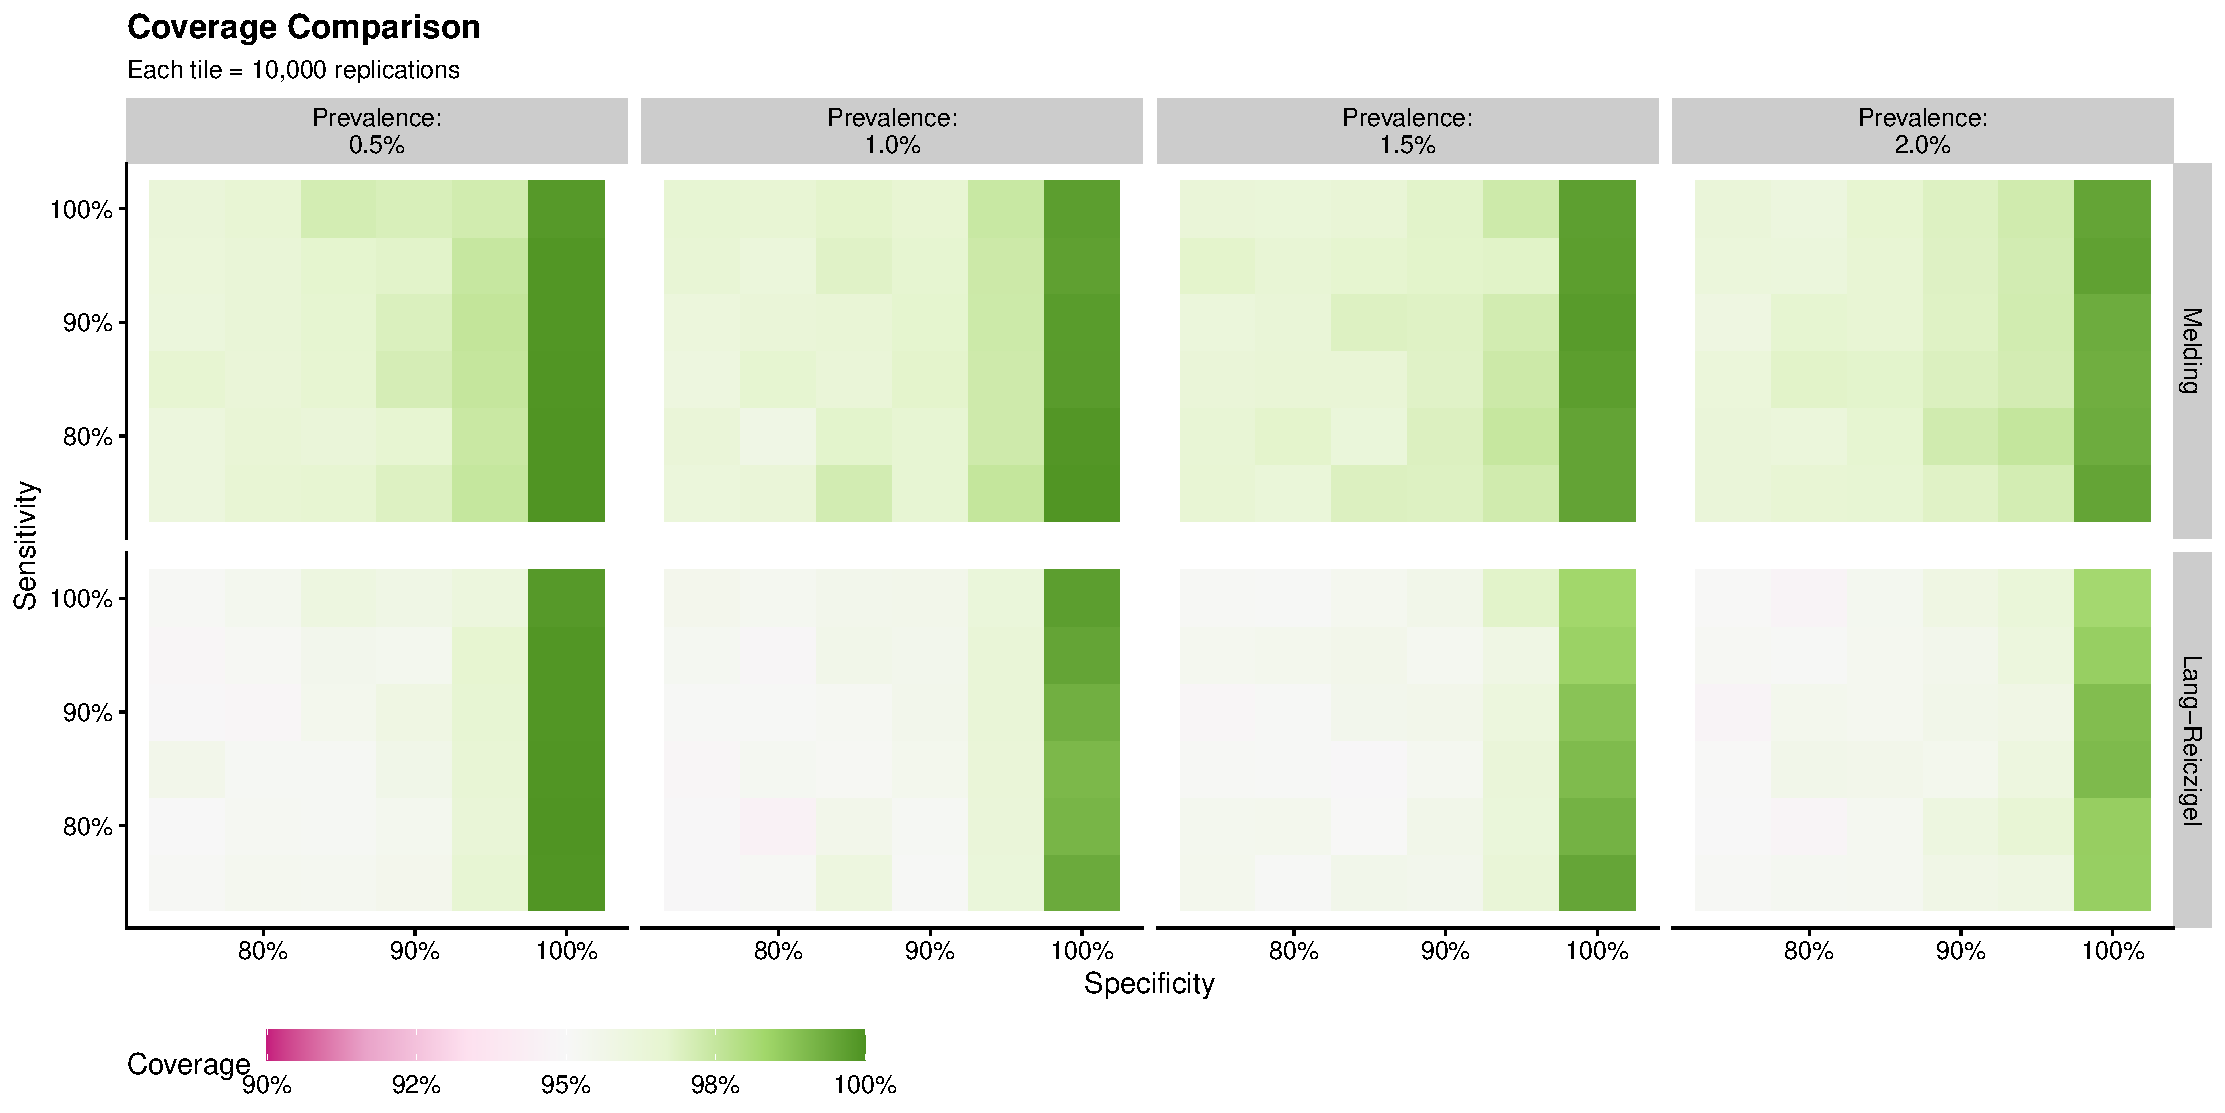
\includegraphics[width=0.8\textwidth]{simple_coverage_comparison_plot}
    \caption[Coverage properties for methods estimating prevalence from a simple random sample with an imperfect assay.]{Coverage properties of 95\% confidence intervals for our new method (Melding) and the Lang-Reiczigel method in a variety of settings, each simulated 10,000 times.}
    \label{ch_3:fig:coverage_comparison_plot}
\end{figure}

\begin{figure}
    \centering
    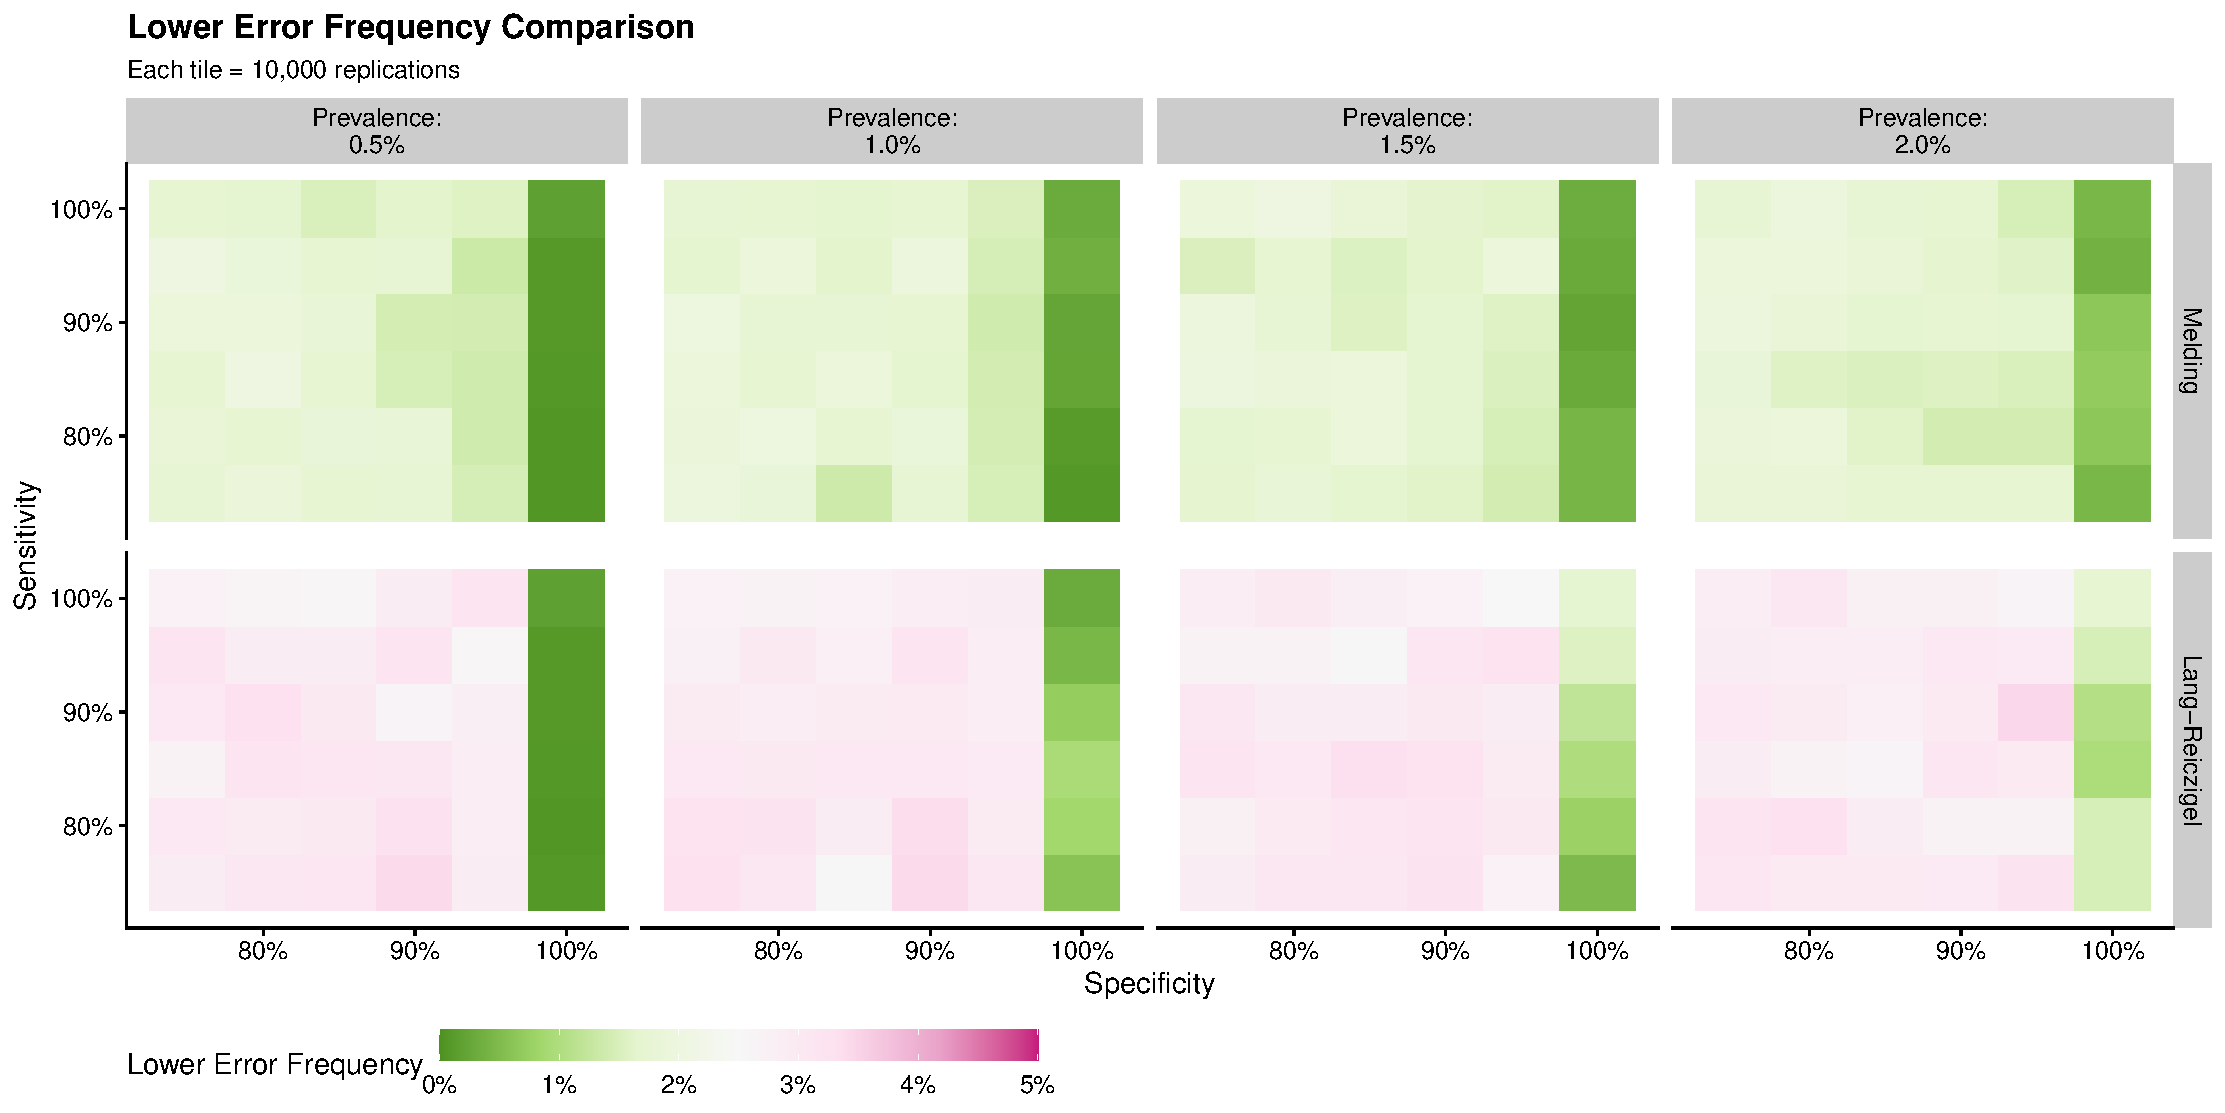
\includegraphics[width=0.8\textwidth]{simple_lower_error_frequency_comparison_plot}
    \caption[Lower error properties for methods estimating prevalence from a simple random sample with an imperfect assay.]{Lower error properties of 95\% confidence intervals for our new method (Melding) and the Lang-Reiczigel method in a variety of settings, each simulated 10,000 times.}
    \label{ch_3:fig:lower_error_frequency_comparison_plot}
\end{figure}

\begin{figure}
    \centering
    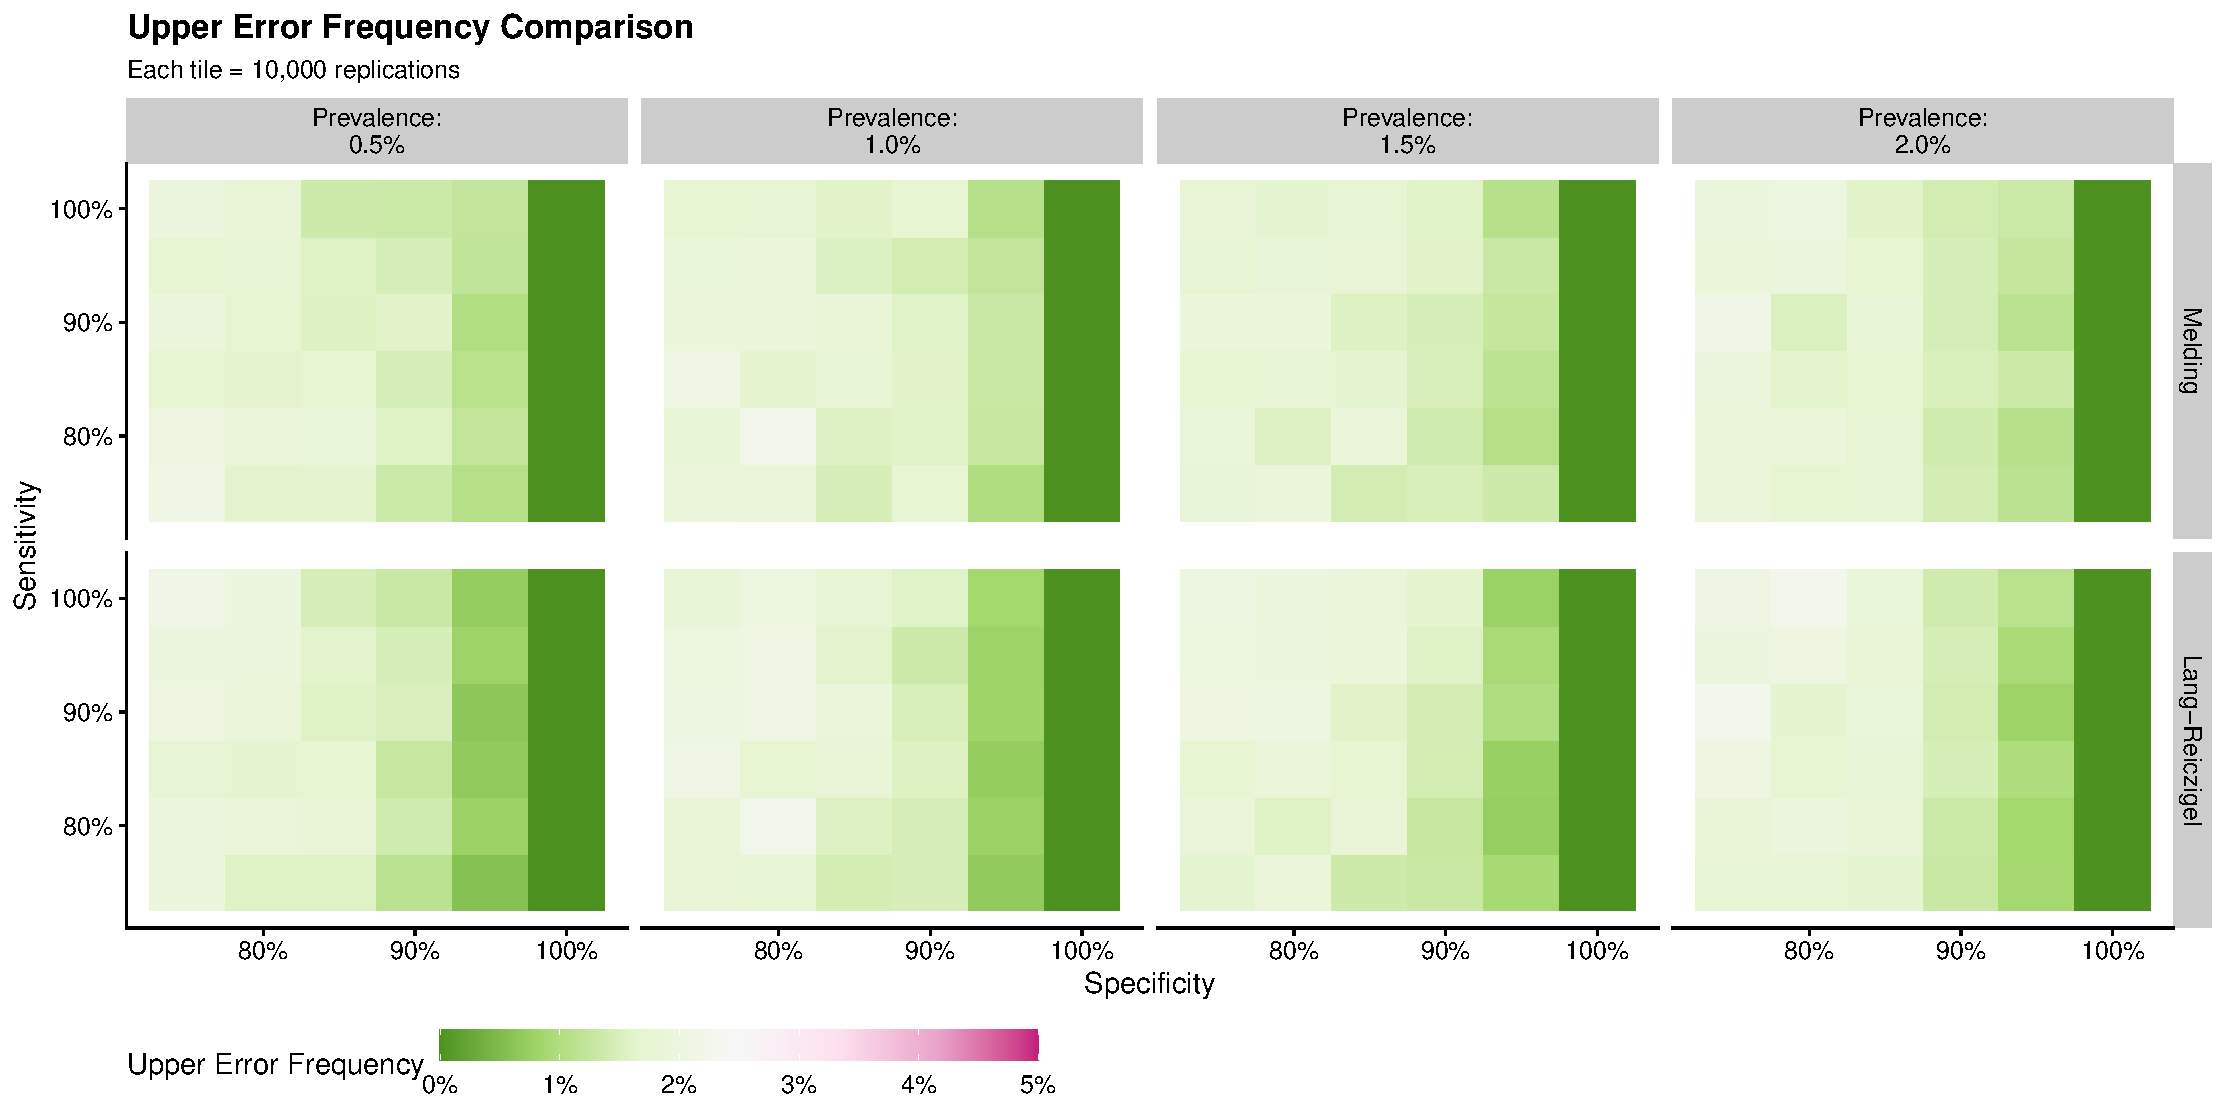
\includegraphics[width=0.8\textwidth]{simple_upper_error_frequency_comparison_plot}
    \caption[Upper error properties for methods estimating prevalence from a simple random sample with an imperfect assay.]{Upper error properties of 95\% confidence intervals for our new method (Melding) and the Lang-Reiczigel method in a variety of settings, each simulated 10,000 times.}
    \label{ch_3:fig:upper_error_frequency_comparison_plot}
\end{figure}

Figure~\ref{ch_3:fig:coverage_comparison_plot} shows that, when specificity is less than perfect, the Lang-Reiczigel method achieves approximately nominal coverage, while the melding method is slightly more conservative, generally demonstrating 96\%-97\% coverage with 95\% confidence intervals.
When specificity is 100\%, both methods are very conservative, achieving nearly 100\% coverage.
For a more nuanced depiction of each method's properties, we separate the overall coverage into lower and upper errors.
Figure~\ref{ch_3:fig:upper_error_frequency_comparison_plot} shows that both methods make upper errors with roughly the same frequency.
Figure~\ref{ch_3:fig:lower_error_frequency_comparison_plot} demonstrates that while the melding procedure bounds the lower error frequency below 2.5\%, the Lang-Reiczigel method generally has lower error frequency above 2.5\%.
Each of these behaviors may be undesirable, depending on the context in which the methods are applied.
For applications in which there is a need to bound the lower errors, the melding method appears to be superior.


\subsection{Estimating Prevalence from a Weighted Sample with a Perfect Assay}
\label{ch_3:sim-perfect}
We compare the wsPoisson method to the more traditional Dean-Pagano modification of the Agresti-Coull (DPAC) method and the Korn-Graubard (KG) method for survey proportions in a variety of settings.
Our simulations examine varying levels of disease prevalence (0.5\% or 5\%), different types of survey designs (50 sampling strata with 200 subjects each or 8000 individuals, each with their own weight), distributions of weights among the sampling strata or individuals (coefficient of variation from approximately 0\% to nearly 600\%), and the number and weights of sampling strata with non-zero prevalence.
For each combination of prevalence \( p \), and group type, up to 500 sets of weights are simulated.
These 500 sets of weights are designed to span a range of coefficients of variation.
For a target coefficient of variation, \( v \), \( n \) weights (\(w_i\)) are simulated by generating \( n \) samples from a \( \text{Beta} \left(\frac{1}{v^2} - \frac{1}{nv^2} - \frac{1}{n}, \frac{n-1}{v^2} - \frac{n-1}{nv^2} - \frac{n-1}{n} \right) \) distribution and normalizing so that \( \sum_{i=1}^n w_i = 1 \).
This assures that the coefficient of variation among these weights is approximately \( v \).
Then, certain weights are chosen to have non-zero prevalence (5\%, 25\%, or 75\% distributed either among the highest weights, lowest weights, or distributed uniformly).
These weights with non-zero prevalence are given a prevalence such that \( \sum_{i=1}^n w_i \theta_i = p \).
For each simulated set of parameters and weights, 10,000 data sets are simulated and assessed.

The coverage properties for these simulations are presented in Figures~\ref{ch_3:fig:perfect_coverage_50_groups_0_005_prev}--\ref{ch_3:fig:perfect_coverage_8000_groups_0_05_prev}.
Additional properties for these simulations are presented in Figures~\ref{ch_3:fig:perfect_lower_error_frequency_50_groups_0_005_prev}--\ref{ch_3:fig:perfect_confidence_interval_width_8000_groups_0_05_prev}.

From Figures~\ref{ch_3:fig:perfect_coverage_50_groups_0_005_prev}--\ref{ch_3:fig:perfect_coverage_8000_groups_0_05_prev}, we note that the two competitor methods generally exhibit lower coverage as the coefficient of variation among the weights increases.
In Figure~\ref{ch_3:fig:perfect_coverage_50_groups_0_005_prev}, this coverage falls below 60\% when the prevalence is very low and is concentrated among the highest weights, and the coefficient of variation among the weights exceeds 4.
Uniform distribution of prevalence among the weights, increased overall prevalence, and larger sample sizes among fewer groups all appear to lessen the severity of this problem.
In contrast, the wsPoisson method appears to guarantee coverage in all scenarios.
The wsPoisson method tends to become more conservative when the coefficient of variation among the weights increases, when the other methods can have problems guaranteeing coverage.
In all cases, the wsPoisson method is more conservative than the competitor methods.
In scenarios with higher overall prevalence, the Agresti-Coul and Korn-Graubard methods achieve close to nominal coverage, while the wsPoisson method strongly over-covers.
This is similar to the behavior observed in \citep{FayF:1997} where, in simulations, the overall error rate for the gamma intervals decreased as the variance of the weights increased.
Because our methods appear to be very conservative, with coverage near 100\% in some cases, we present the widths of the confidence intervals in Figures~\ref{ch_3:fig:perfect_confidence_interval_width_50_groups_0_005_prev}--\ref{ch_3:fig:perfect_confidence_interval_width_8000_groups_0_05_prev}.
In scenarios where coefficient of variation among the survey weights is high, the wsPoisson intervals are often two or three times wider than intervals produced by competing methods.


\begin{figure}
\centering
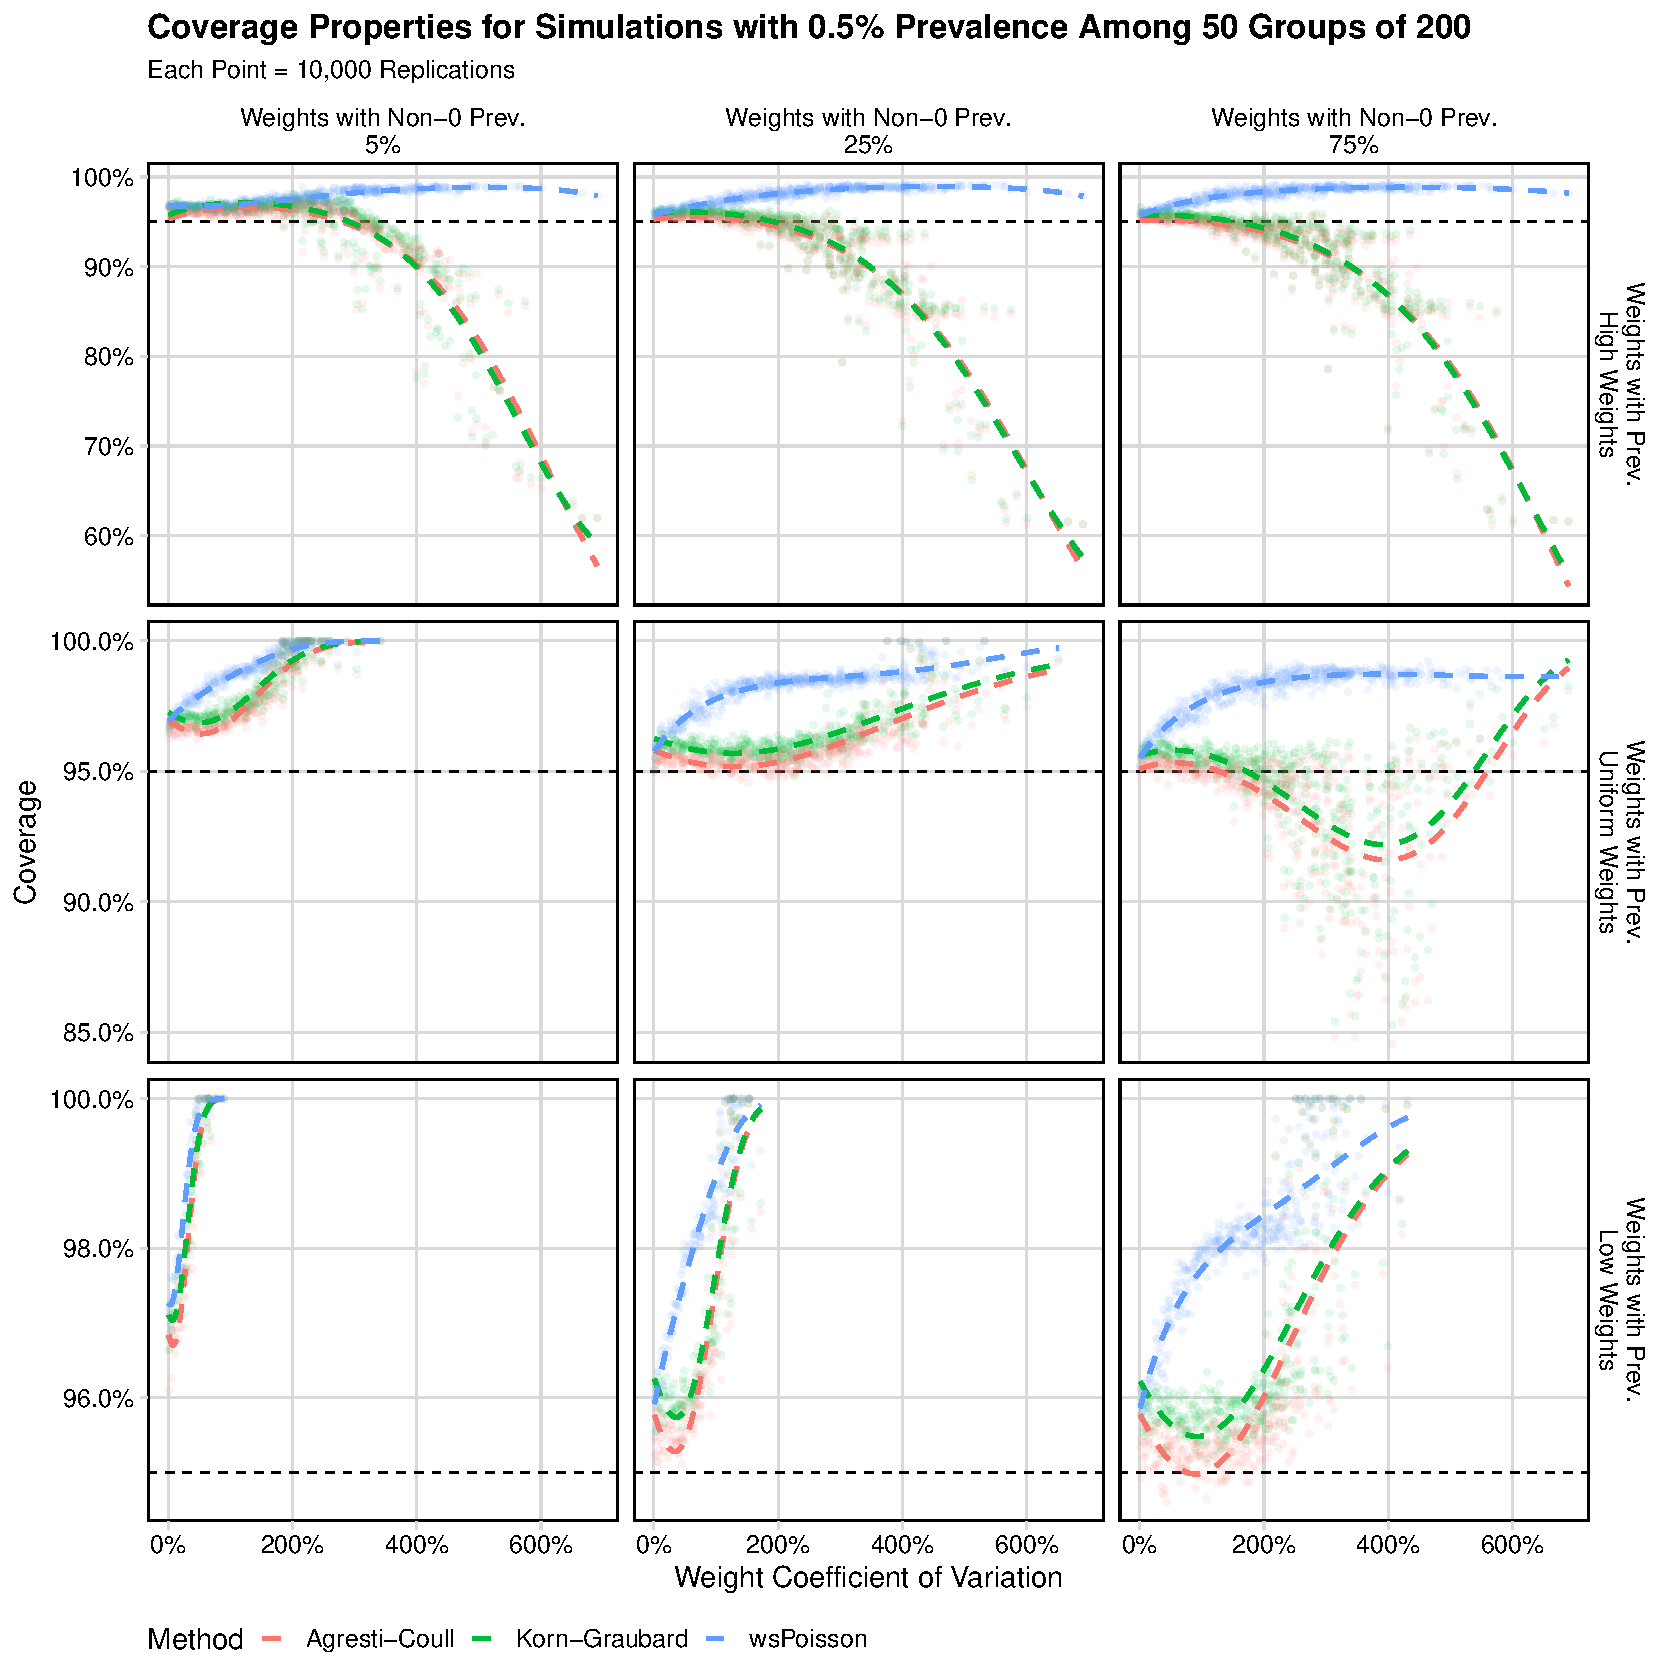
\includegraphics[width=0.8\textwidth]{perfect_coverage_50_groups_0_005_prev}
\caption[Coverage properties for methods estimating prevalence from a weighted sample with a perfect assay (50 groups of 200, 0.5\% population prevalence).]{Coverage properties for the wsPoisson model and two standard methods, the Dean-Pagano modification of the Agresti-Coull method and of the Korn-Graubard method.
Each point represents 10,000 simulations of datasets from a population with 0.5\% prevalence, where 50 groups of 200 people are sampled.
The horizontal dashed line indicates the nominal coverage, 95\%.
Colored dashed lines are estimates from a logistic regression model using quadratic splines.}
\label{ch_3:fig:perfect_coverage_50_groups_0_005_prev}
\end{figure}

\begin{figure}
\centering
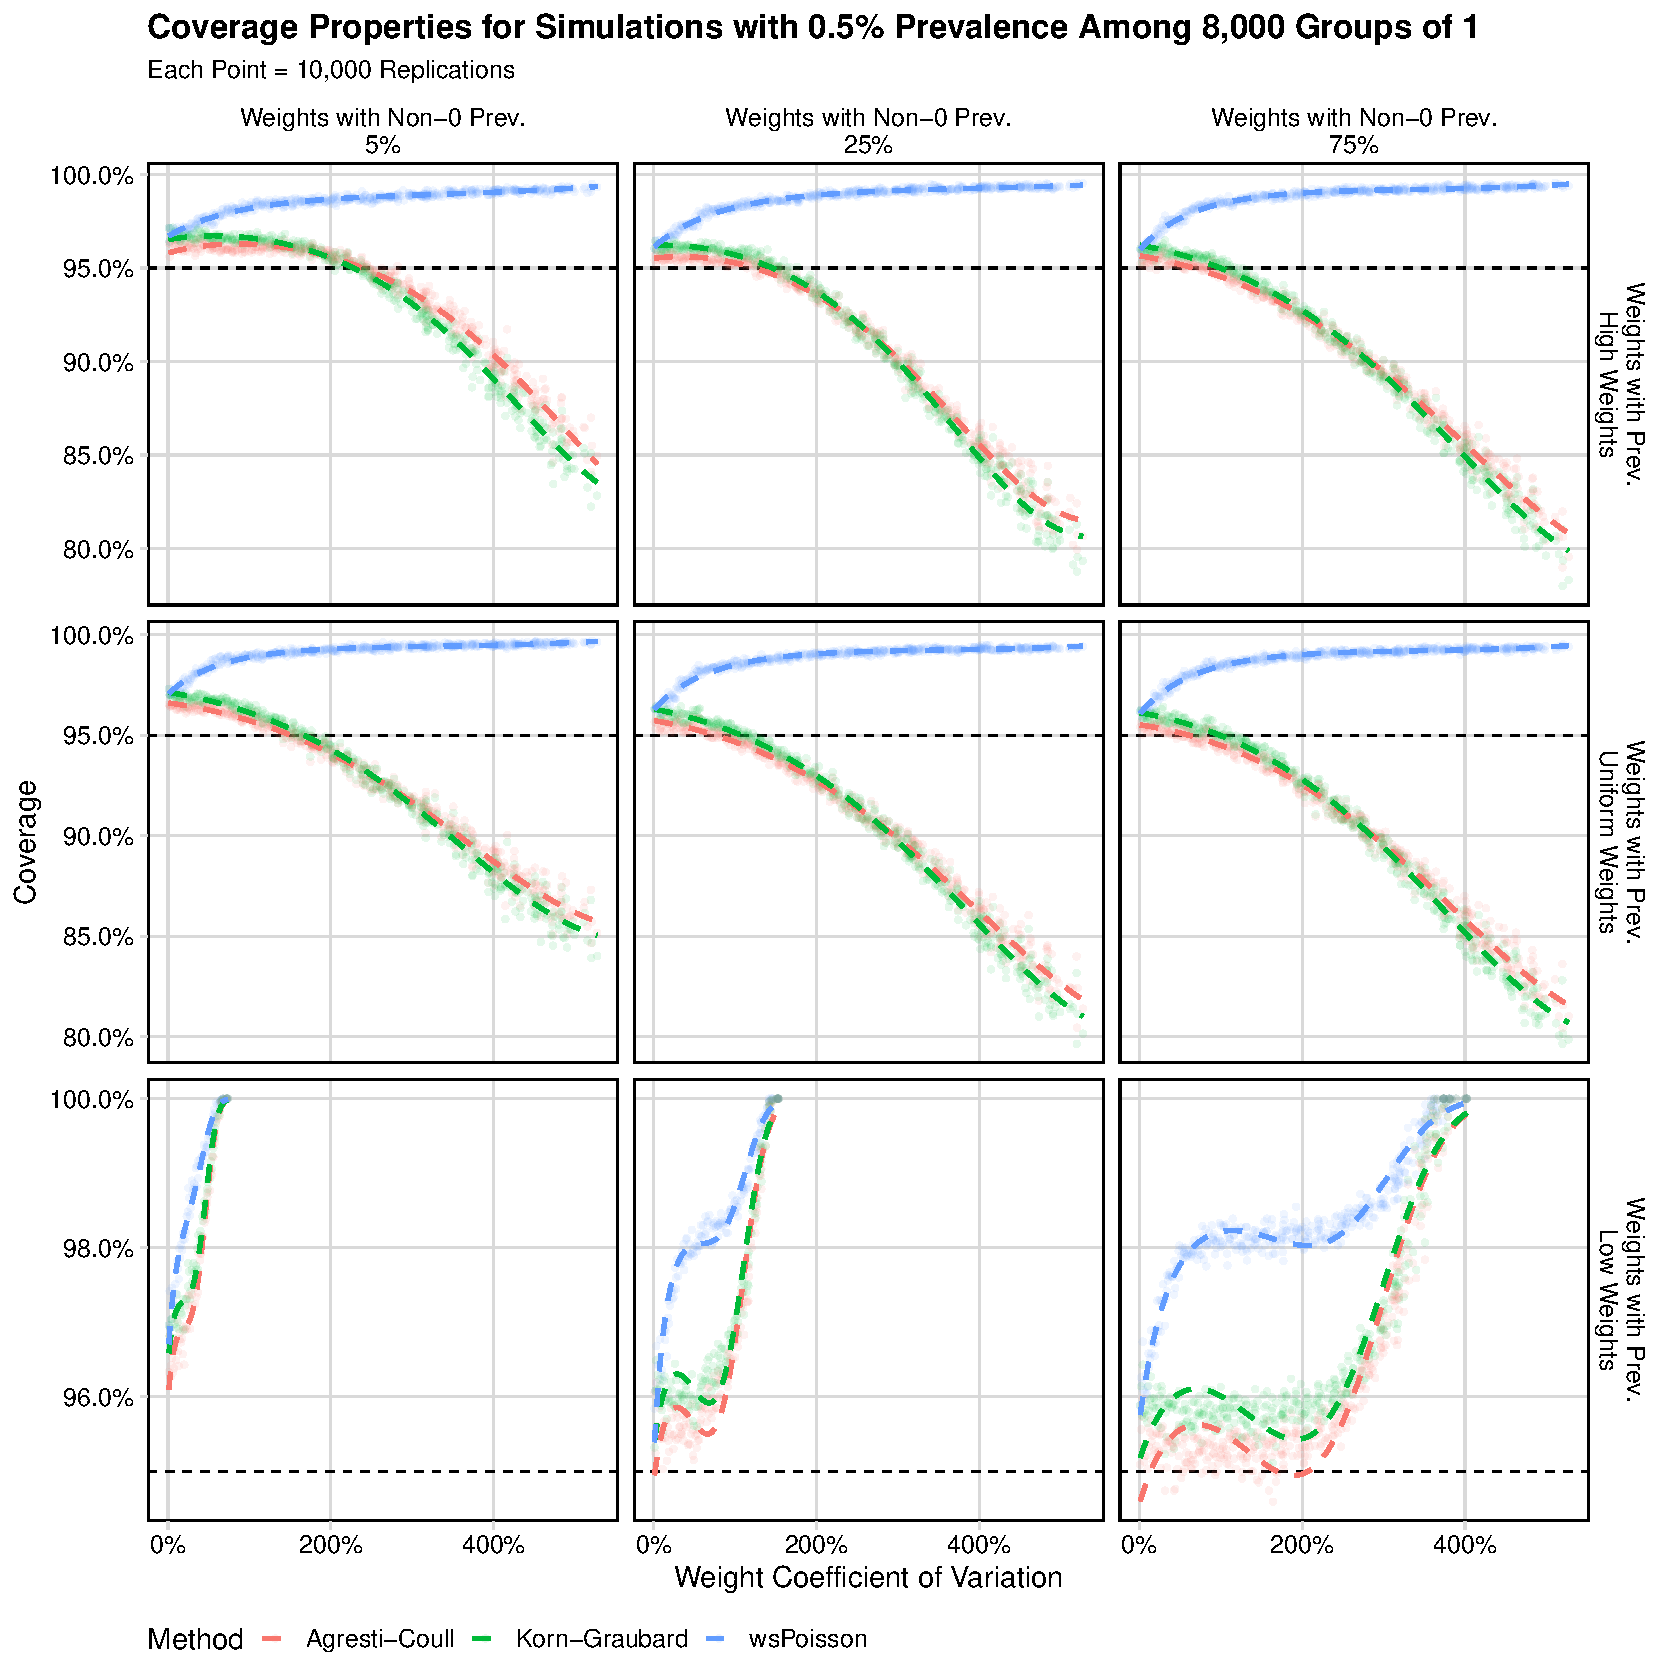
\includegraphics[width=0.8\textwidth]{perfect_coverage_8000_groups_0_005_prev}
\caption[Coverage properties for methods estimating prevalence from a weighted sample with a perfect assay (8000 individuals, 0.5\% population prevalence).]{Coverage properties for the wsPoisson model and two standard methods, the Dean-Pagano modification of the Agresti-Coull method and of the Korn-Graubard method.
Each point represents 10,000 simulations of datasets from a population with 0.5\% prevalence where 8000 individuals are sampled.
The horizontal dashed line indicates the nominal coverage, 95\%.
Colored dashed lines are estimates from a logistic regression model using quadratic splines.}
\label{ch_3:fig:perfect_coverage_8000_groups_0_005_prev}
\end{figure}

\begin{figure}
\centering
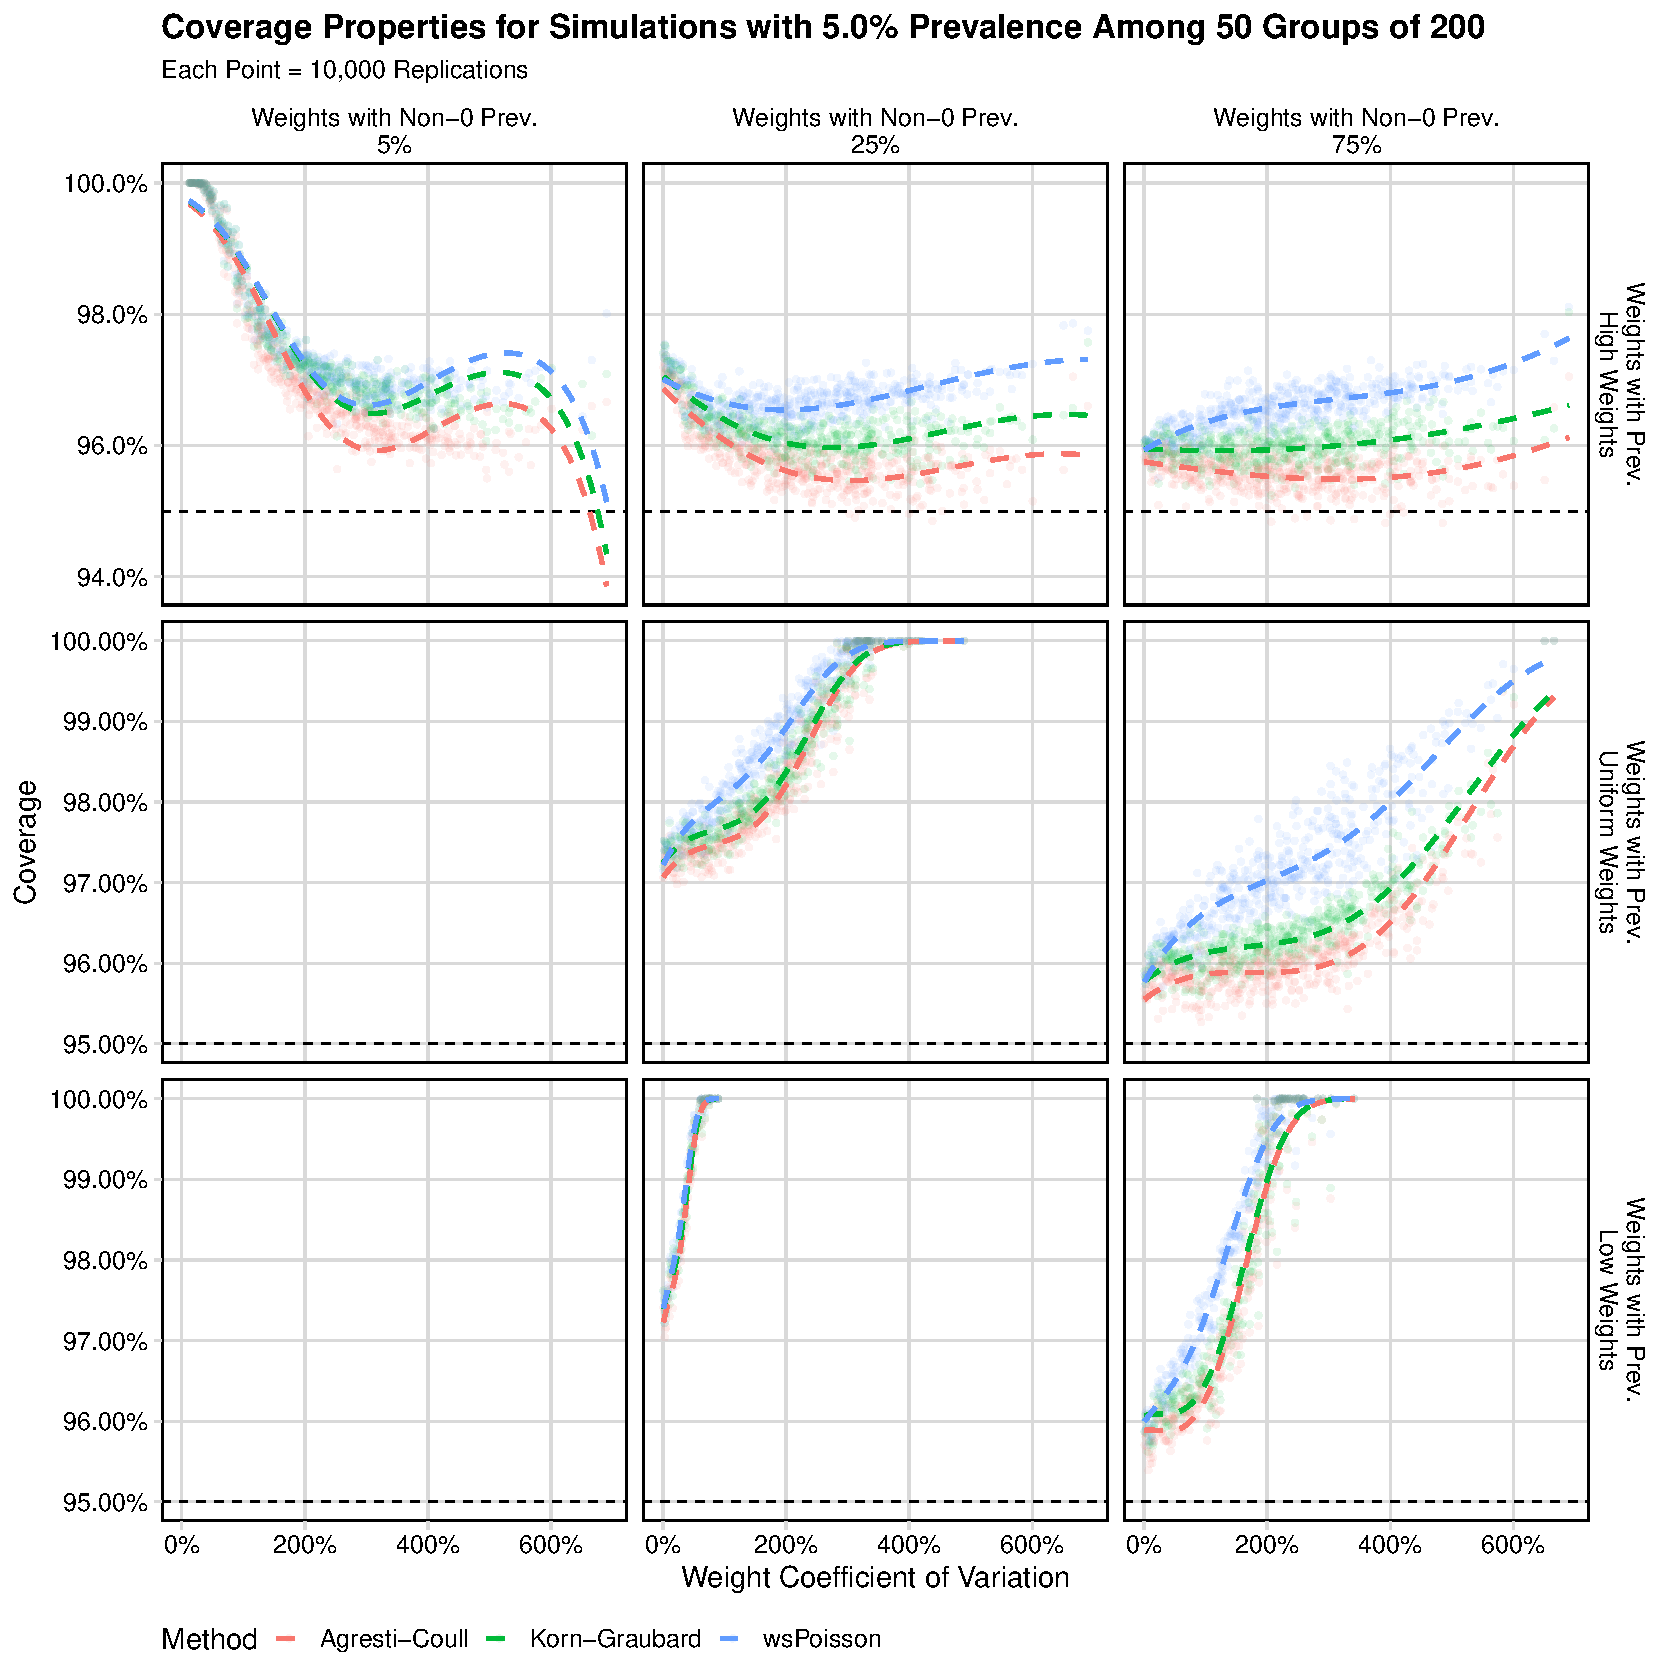
\includegraphics[width=0.8\textwidth]{perfect_coverage_50_groups_0_05_prev}
\caption[Coverage properties for methods estimating prevalence from a weighted sample with a perfect assay (50 groups of 200, 5\% population prevalence).]{Coverage properties for the wsPoisson model and two standard methods, the Dean-Pagano modification of the Agresti-Coull method and of the Korn-Graubard method.
Each point represents 10,000 simulations of datasets from a population with 5\% prevalence, where 50 groups of 200 people are sampled.
The horizontal dashed line indicates the nominal coverage, 95\%.
Colored dashed lines are estimates from a logistic regression model using quadratic splines.}
\label{ch_3:fig:perfect_coverage_50_groups_0_05_prev}
\end{figure}

\begin{figure}
\centering
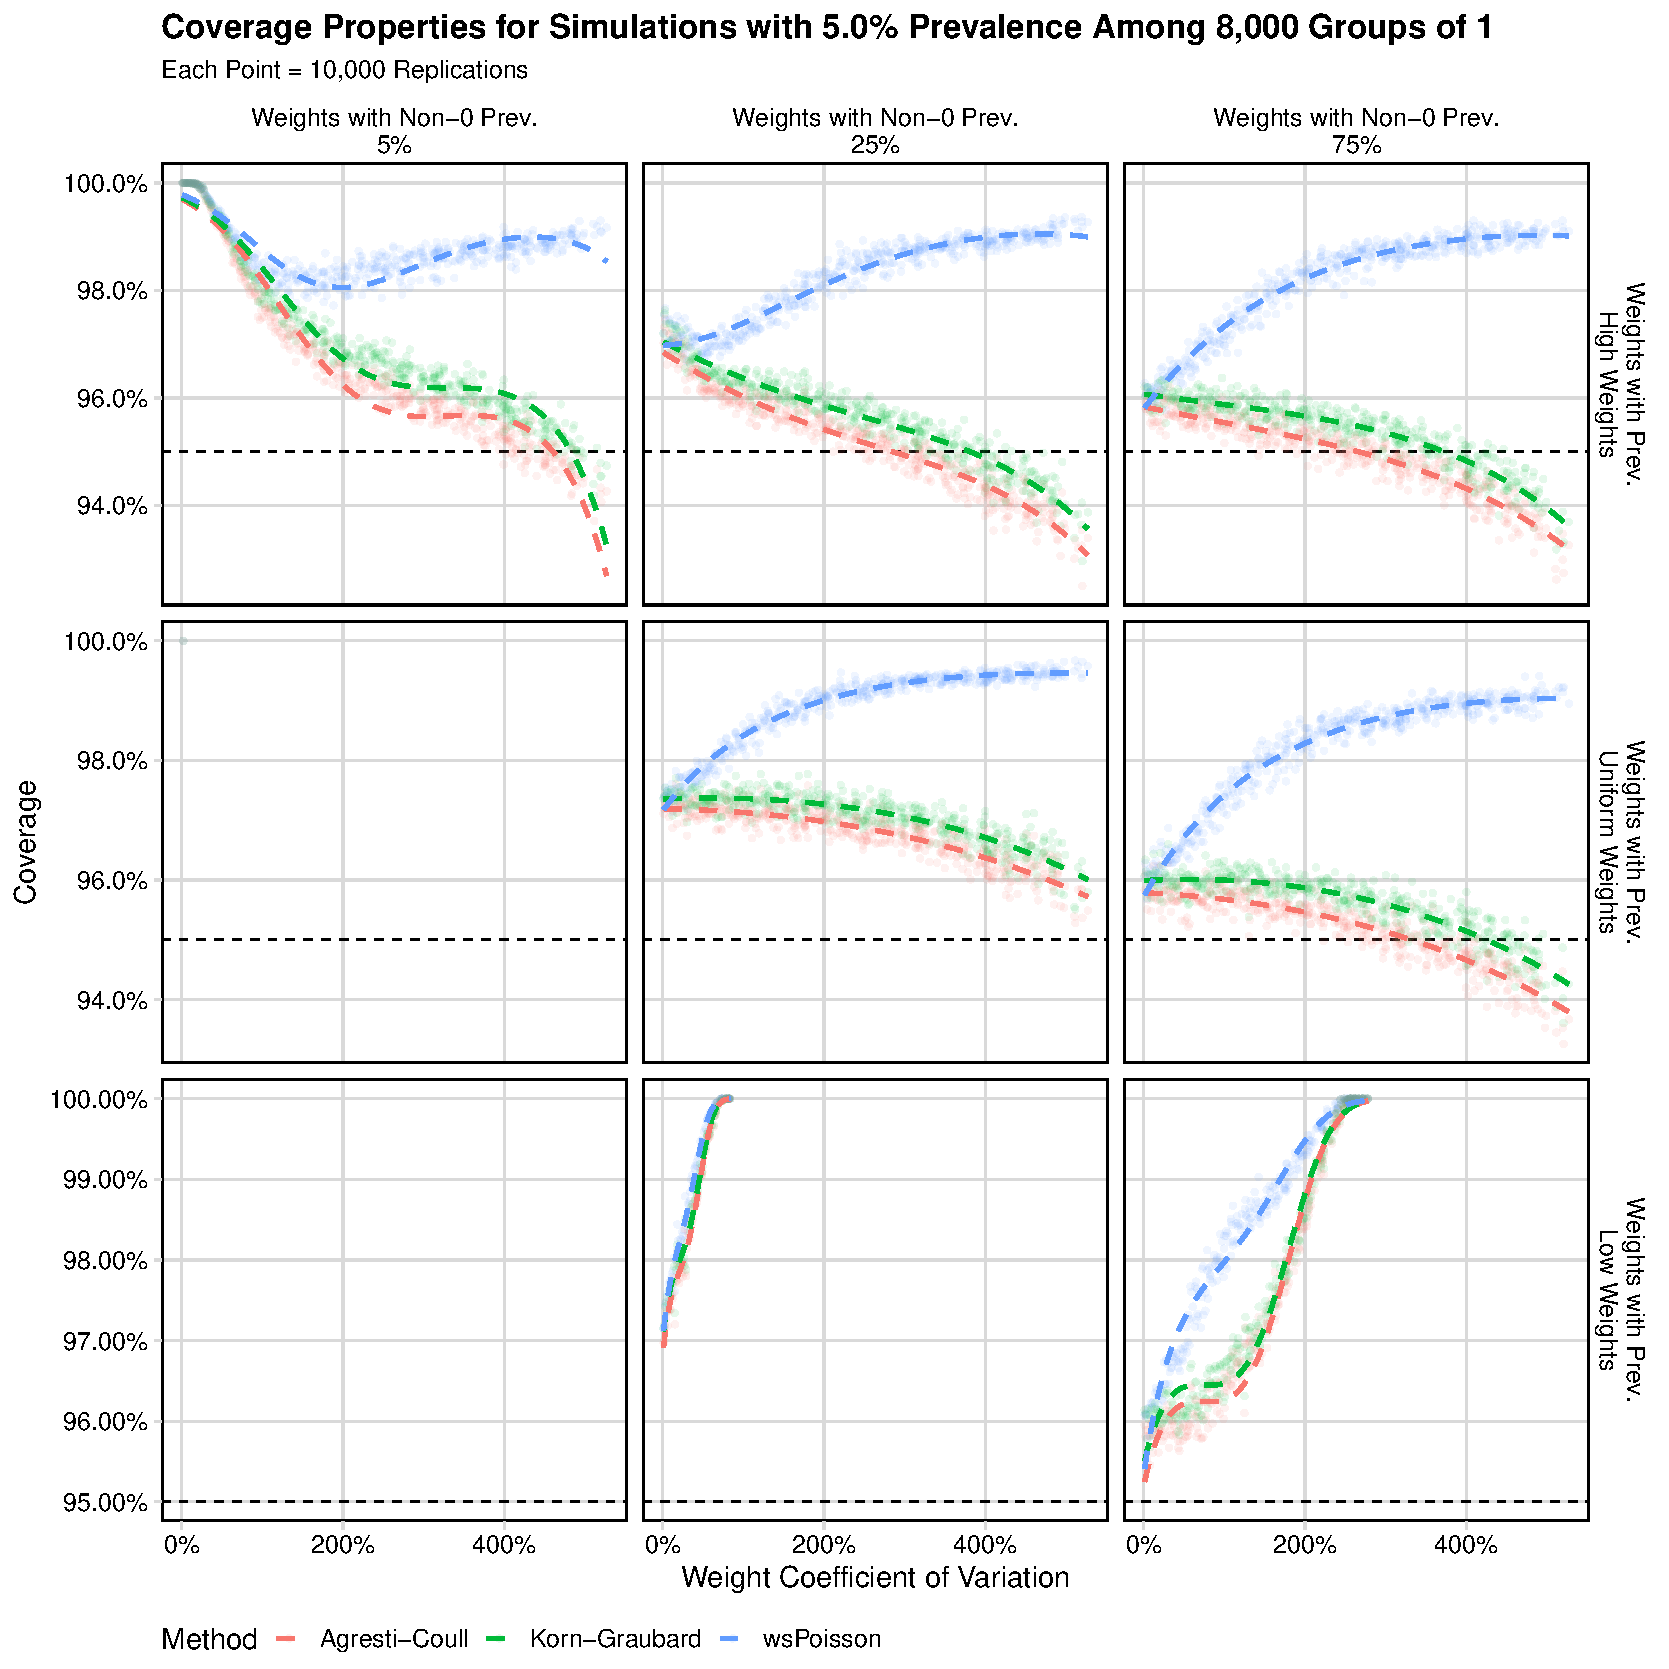
\includegraphics[width=0.8\textwidth]{perfect_coverage_8000_groups_0_05_prev}
\caption[Coverage properties for methods estimating prevalence from a weighted sample with a perfect assay (8000 individuals, 5\% population prevalence).]{Coverage properties for the wsPoisson model and two standard methods, the Dean-Pagano modification of Agresti-Coull and Korn-Graubard.
Each point represents 10,000 simulations of datasets from a population with 5\% prevalence where 8000 individuals are sampled.
The horizontal dashed line indicates the nominal coverage, 95\%.
Colored dashed lines are estimates from a logistic regression model using quadratic splines.}
\label{ch_3:fig:perfect_coverage_8000_groups_0_05_prev}
\end{figure}


\subsection{Estimating Prevalence from a Weighted Sample with an Imperfect Assay}

We compare properties of our melded confidence interval, WprevSeSp Poisson, to another melded confidence interval method, WprevSeSp Binomial, for cases with weighted samples and imperfect assays.
The methods are assessed in several simulated scenarios with varying levels of disease prevalence (0.5\% or 5\%), types of groups surveyed (50 groups of 200 subjects each or 8000 groups of 1 subject), distributions of weights among the groups (coefficient of variation from approximately 0\% to nearly 600\%), the number of groups with non-zero prevalence, and the specificity of the assay (80\% - 100\%).
In each scenario, the assay has 95\% sensitivity.
Each scenario creates up to 500 new sets of weights and $\theta_i$ parameters (as in Section~\ref{ch_3:sim-perfect}), and each of those is simulated 10,000 times, with new prevalence, sensitivity, and specificity surveys generated and 95\% confidence intervals are created.
Modeled after the study of \citet{Kali:2021}, the simulated sensitivity is assessed based on 60 tests, while specificity is based on 300 tests.

The coverage properties for these simulations are presented in Figures~\ref{ch_3:fig:imperfect_coverage_50_groups_0_005_prev}--\ref{ch_3:fig:imperfect_coverage_8000_groups_0_05_prev}.
Additional properties for these simulations are presented in Figures~\ref{ch_3:fig:imperfect_lower_error_frequency_50_groups_0_05_prev}--\ref{ch_3:fig:imperfect_confidence_interval_width_8000_groups_0_05_prev}.

\begin{figure}
\centering
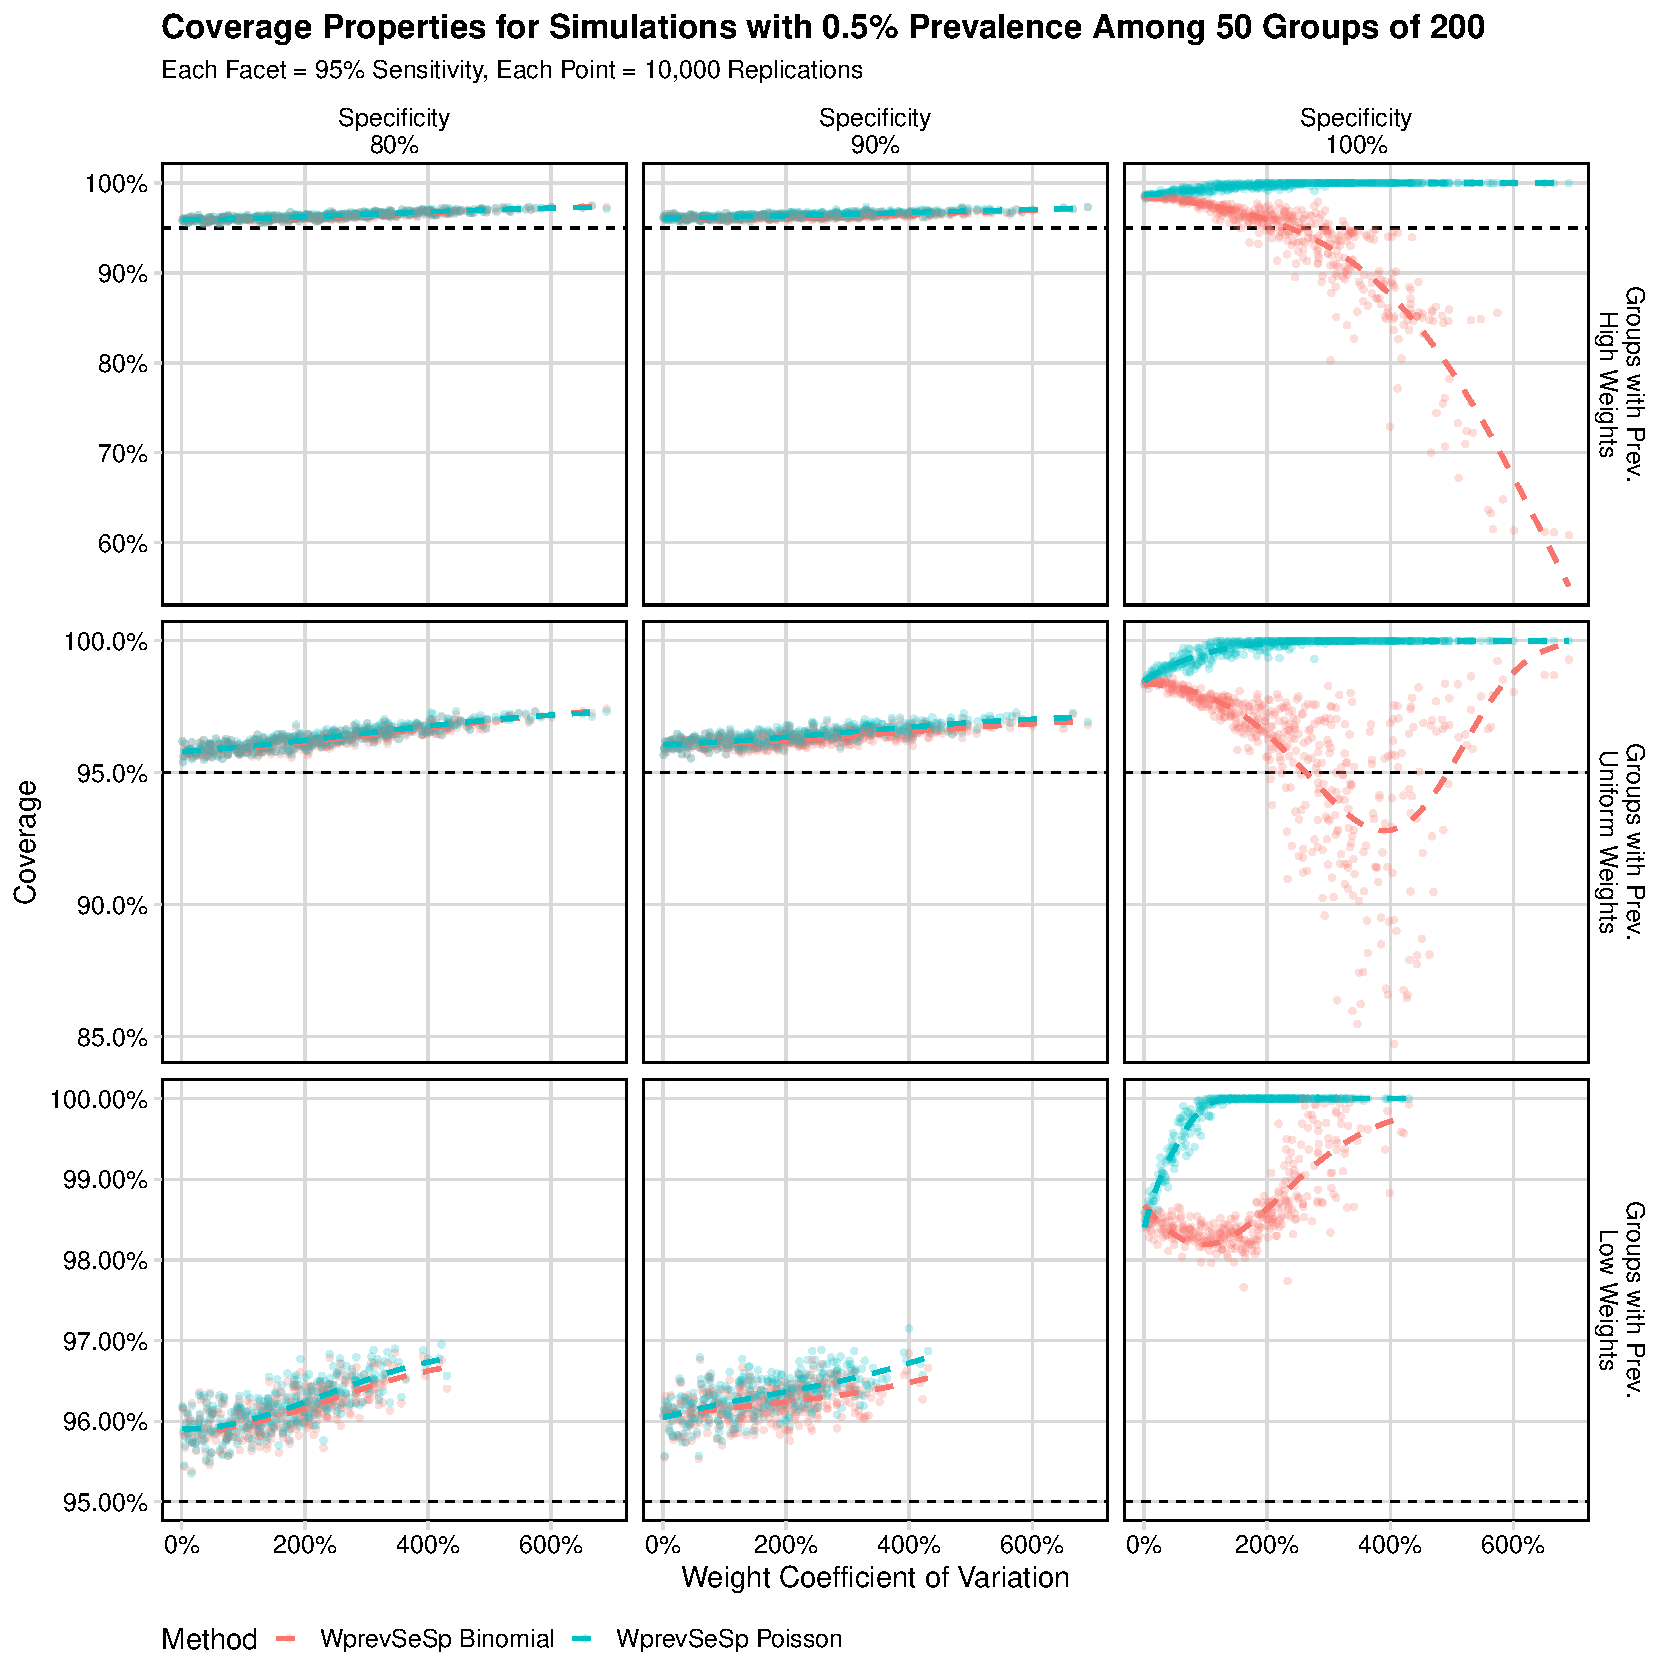
\includegraphics[width=0.8\textwidth]{imperfect_coverage_50_groups_0_005_prev}
\caption[Coverage properties for methods estimating prevalence from a weighted sample with an imperfect assay (50 groups of 200, 0.5\% population prevalence).]{Coverage properties for the confidence interval procedures, WprevSeSp Binomial and WprevSeSp Poisson.
Each point represents 10,000 simulations of datasets from a population with 0.5\% prevalence, where 50 groups of 200 people are sampled.
Each  also includes simulated results of tests to evaluate the sensitivity and specificity of the assay performed on 60 and 300 individuals, respectively.
The horizontal dashed line indicates the nominal coverage, 95\%.
Colored dashed lines are estimates from a logistic regression model using quadratic splines.}
\label{ch_3:fig:imperfect_coverage_50_groups_0_005_prev}
\end{figure}

\begin{figure}
\centering
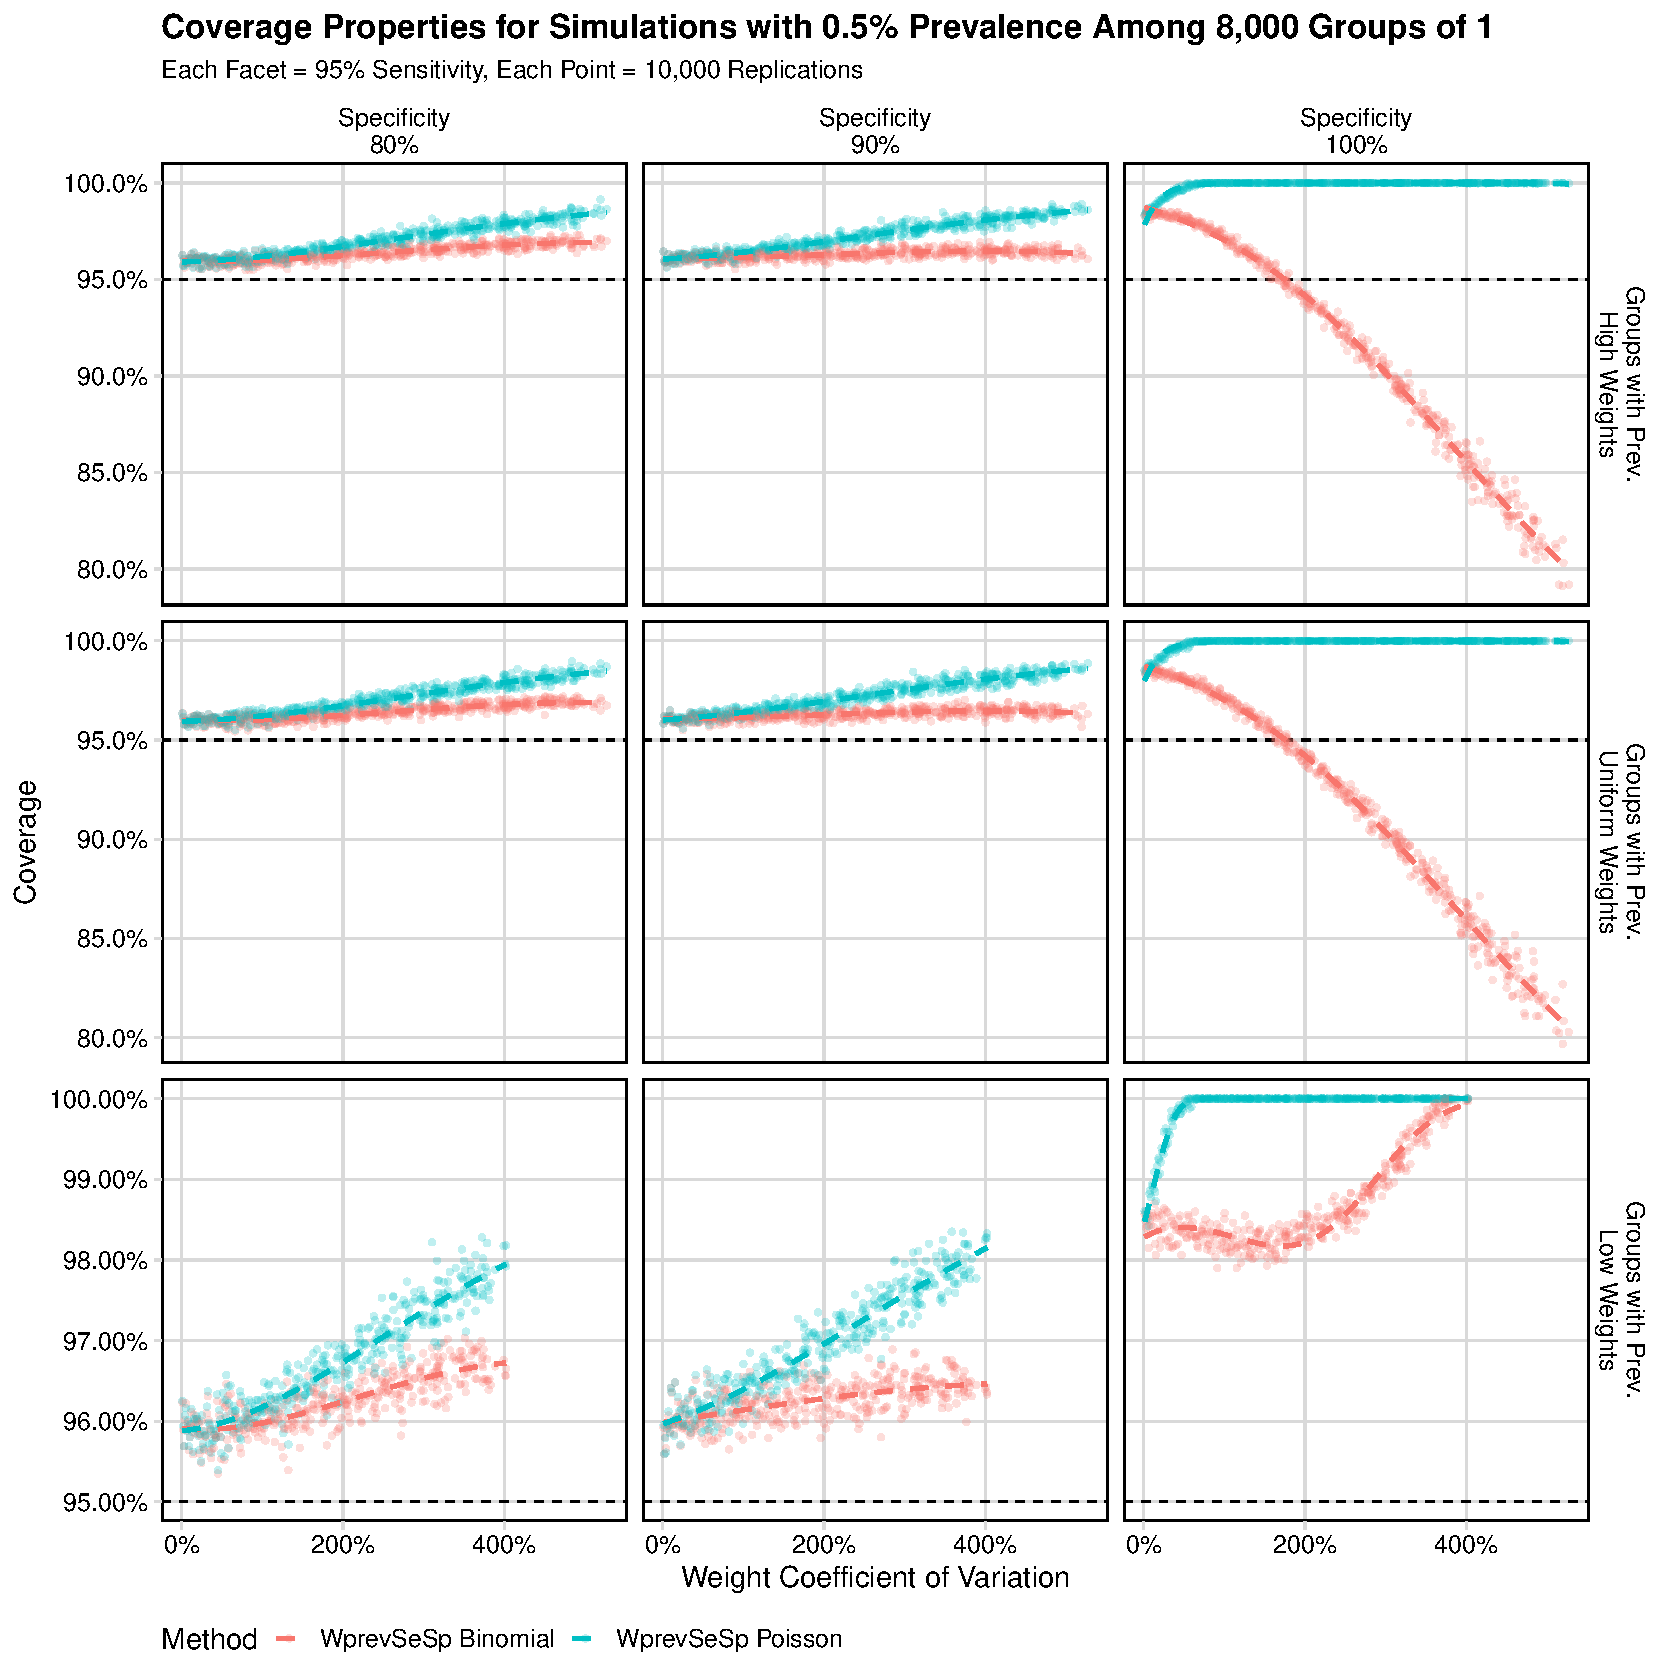
\includegraphics[width=0.8\textwidth]{imperfect_coverage_8000_groups_0_005_prev}
\caption[Coverage properties for methods estimating prevalence from a weighted sample with an imperfect assay (8000 individuals, 0.5\% population prevalence).]{Coverage properties for the confidence interval procedures, WprevSeSp Binomial and WprevSeSp Poisson.
Each point represents 10,000 simulations of datasets from a population with 0.5\% prevalence where 8000 individuals are sampled.
Each dataset also includes simulated results of tests to evaluate the sensitivity and specificity of the assay performed on 60 and 300 individuals, respectively.
The horizontal dashed line indicates the nominal coverage, 95\%.
Colored dashed lines are estimates from a logistic regression model using quadratic splines.}
\label{ch_3:fig:imperfect_coverage_8000_groups_0_005_prev}
\end{figure}

\begin{figure}
\centering
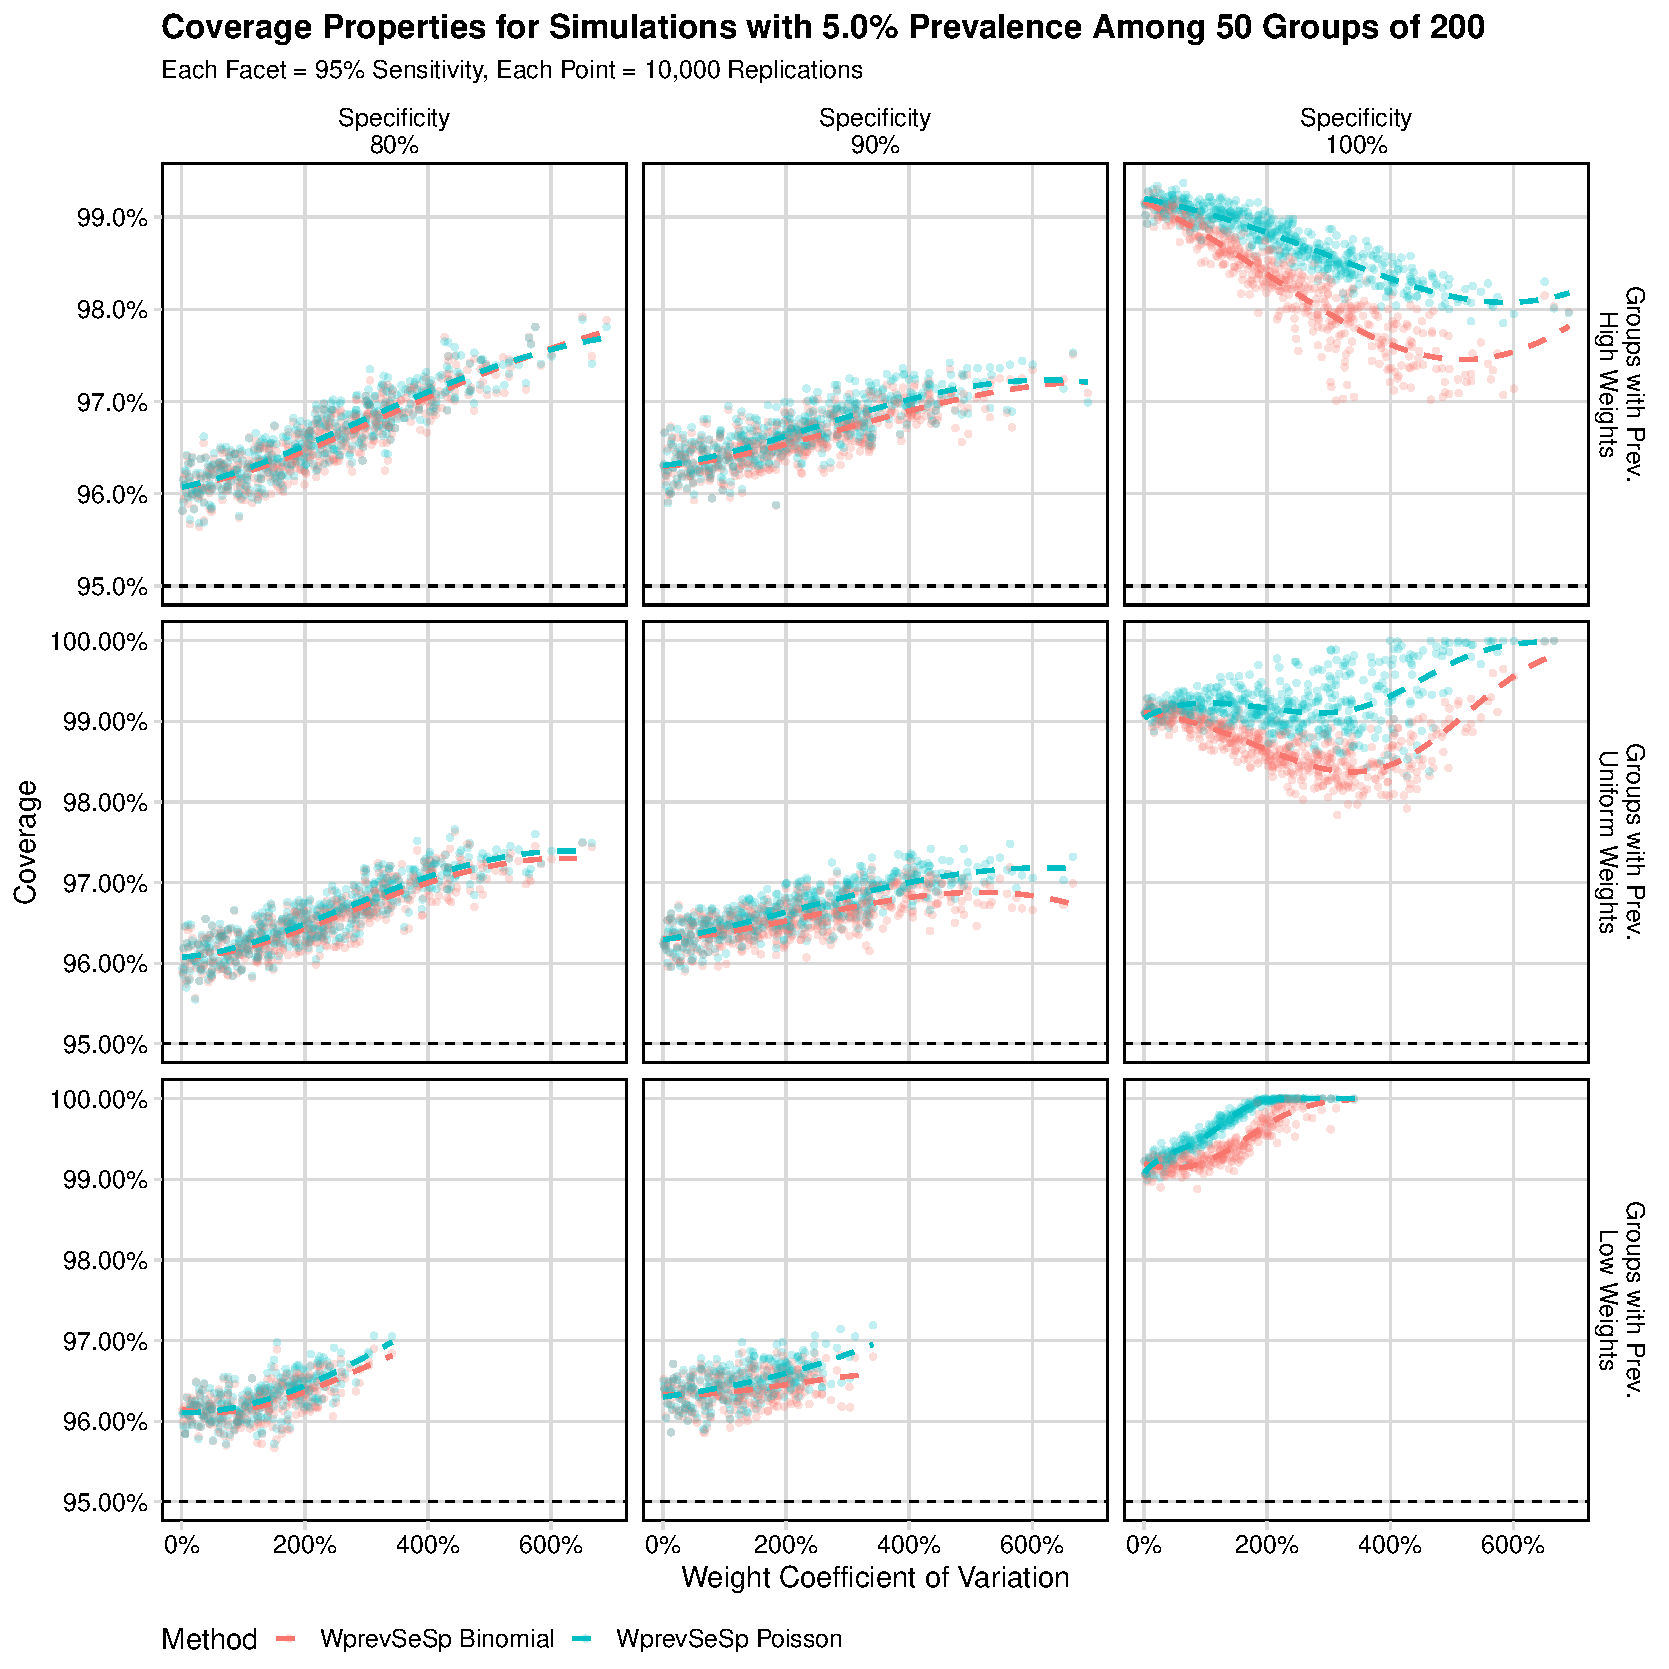
\includegraphics[width=0.8\textwidth]{imperfect_coverage_50_groups_0_05_prev}
\caption[Coverage properties for methods estimating prevalence from a weighted sample with an imperfect assay (50 groups of 200, 5\% population prevalence).]{Coverage properties for the confidence interval procedures, WprevSeSp Binomial and WprevSeSp Poisson.
Each point represents 10,000 simulations of datasets from a population with 5\% prevalence, where 50 groups of 200 people are sampled.
Each dataset also includes simulated results of tests to evaluate the sensitivity and specificity of the assay performed on 60 and 300 individuals, respectively.
The horizontal dashed line indicates the nominal coverage, 95\%.
Colored dashed lines are estimates from a logistic regression model using quadratic splines.}
\label{ch_3:fig:imperfect_coverage_50_groups_0_05_prev}
\end{figure}

\begin{figure}
\centering
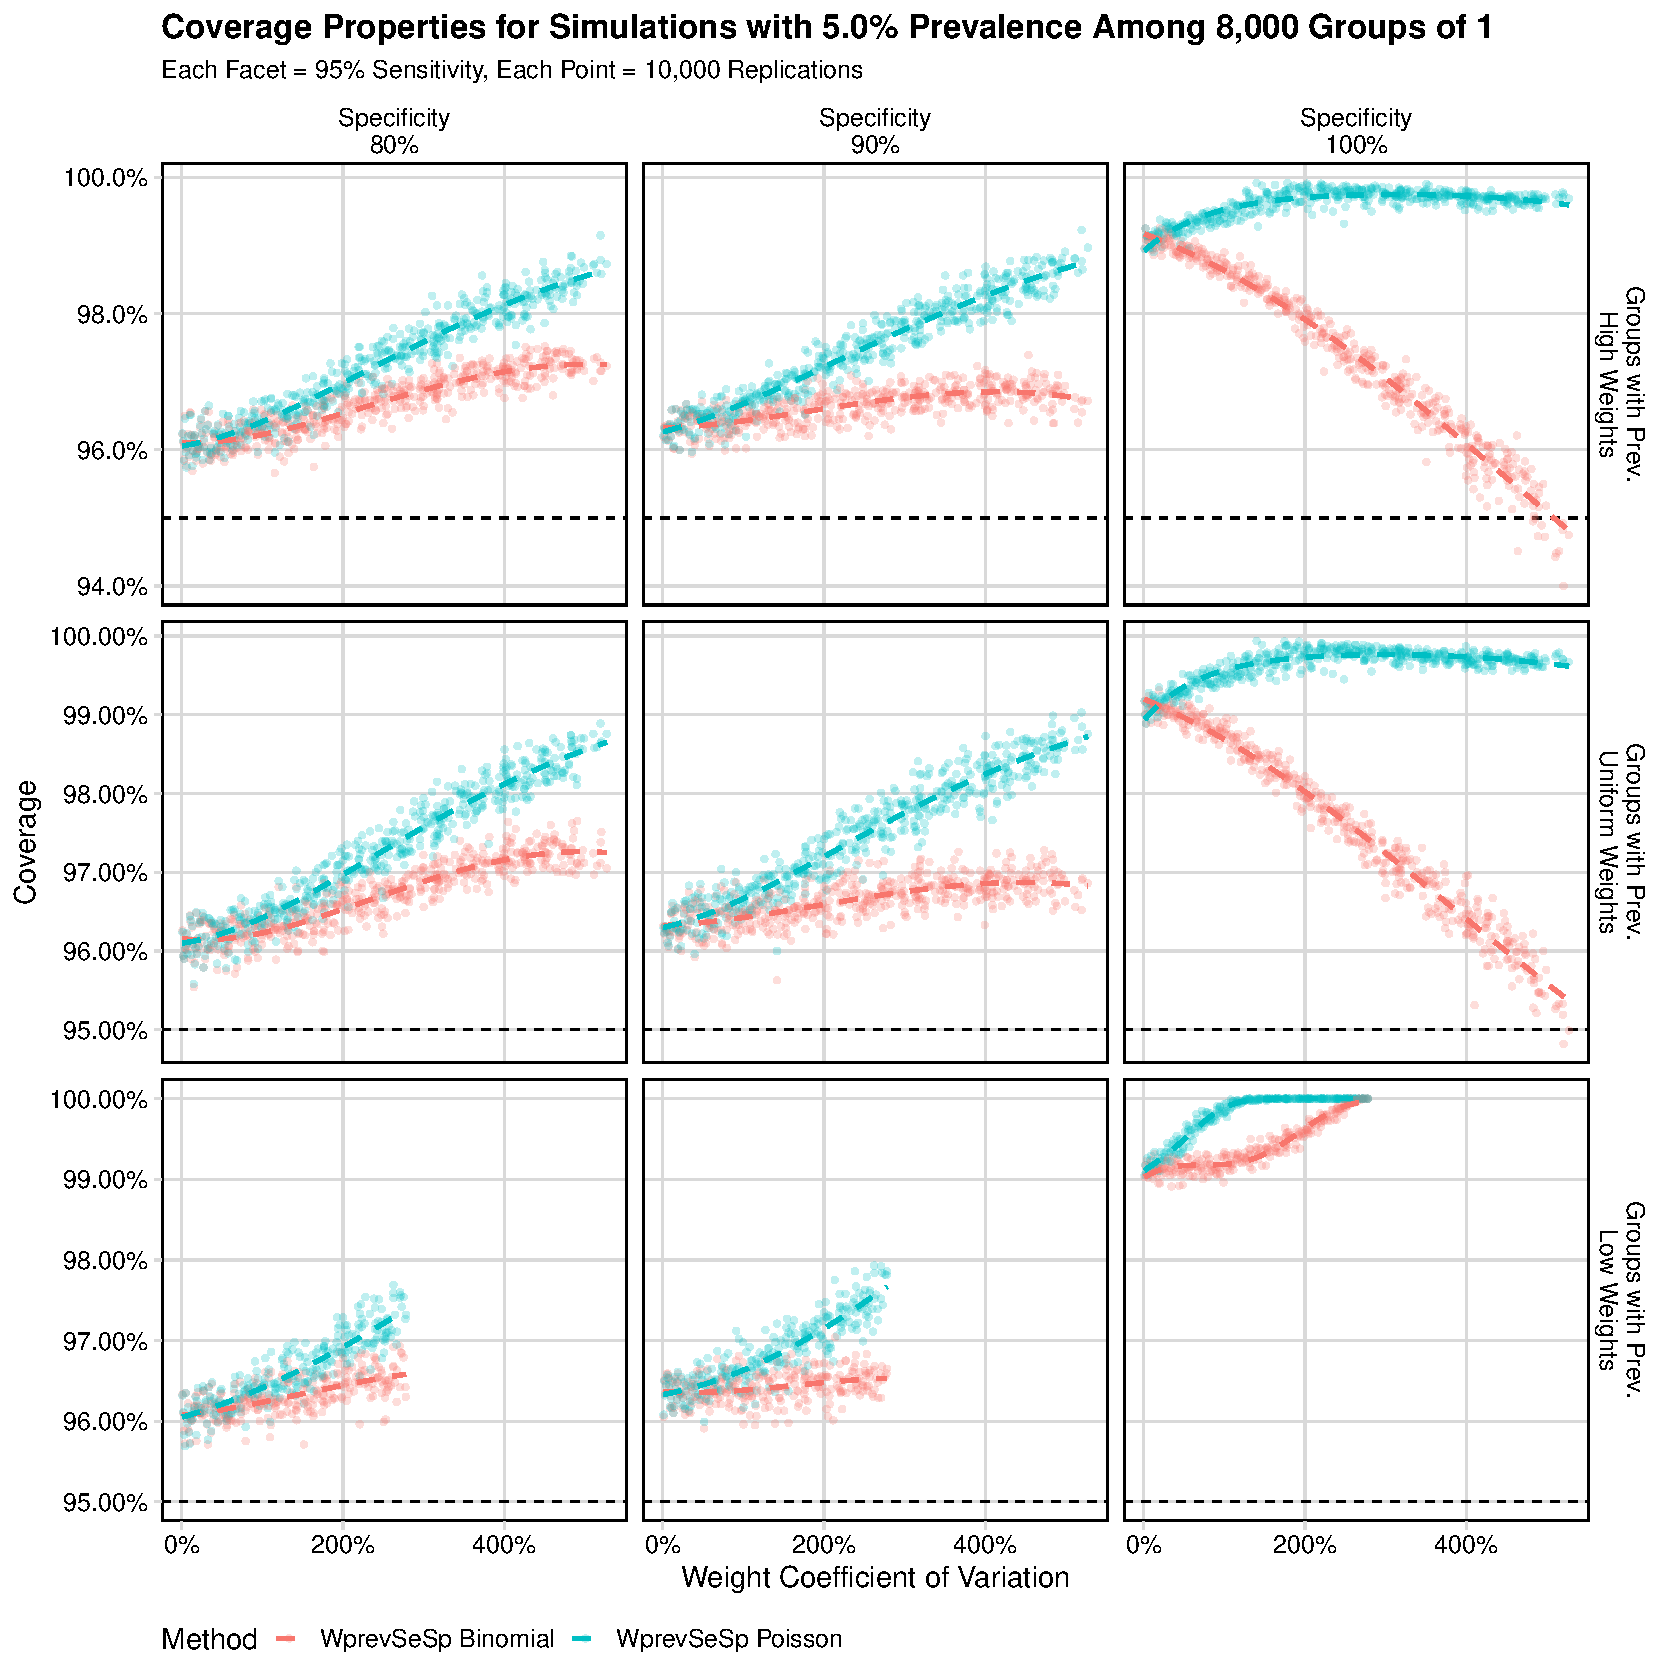
\includegraphics[width=0.8\textwidth]{imperfect_coverage_8000_groups_0_05_prev}
\caption[Coverage properties for methods estimating prevalence from a weighted sample with an imperfect assay (8000 individuals, 5\% population prevalence).]{Coverage properties for the confidence interval procedures, WprevSeSp Binomial and WprevSeSp Poisson.
Each point represents 10,000 simulations of datasets from a population with 5\% prevalence where 8000 individuals are sampled.
Each dataset also includes simulated results of tests to evaluate the sensitivity and specificity of the assay performed on 60 and 300 individuals, respectively.
The horizontal dashed line indicates the nominal coverage, 95\%.
Colored dashed lines are estimates from a logistic regression model using quadratic splines.}
\label{ch_3:fig:imperfect_coverage_8000_groups_0_05_prev}
\end{figure}

Based on Figures~\ref{ch_3:fig:imperfect_lower_error_frequency_50_groups_0_05_prev}--\ref{ch_3:fig:imperfect_upper_error_frequency_8000_groups_0_05_prev}, we note that, in most settings, the two melding procedures result in conservative confidence intervals, often nearing 100\% coverage.
With perfect specificity, the WprevSeSp Binomial method fails to maintain nominal coverage when the coefficient of variation among the weights is high and specificity is perfect.
In the other scenarios tested, the WprevSeSp Binomial generally achieves closer to nominal coverage than the WprevSeSp Poisson, which strongly over-covers.
Our proposed WprevSeSp Poisson method maintains or exceeds the desired coverage in all scenarios.
In these scenarios, we also assess properties of the wsPoisson procedure, which does not account for the imperfect assay.
This method results in approximately 0\% coverage in any scenarios where specificity is less than perfect.
For this reason, results from that method are omitted in the figures.
Because both WprevSeSp methods appear to be very conservative, with coverage near 100\% in some cases, we present the widths of the confidence intervals in Figures~\ref{ch_3:fig:imperfect_confidence_interval_width_50_groups_0_005_prev}--\ref{ch_3:fig:imperfect_confidence_interval_width_8000_groups_0_05_prev}.
The WprevSeSp Binomial and WprevSeSp Poisson methods typically produce wide intervals of approximately the same size - sometimes as wide as 12\%, even when the true prevalence is 0.05\%.
One notable exception to this is presented in Figure \ref{ch_3:fig:imperfect_confidence_interval_width_8000_groups_0_005_prev}, which shows that for tests with perfect specificity, the WprevSeSP Binomial method produces much narrower confidence intervals than the other method.

\section{Application}
\label{ch_3:sec-Application}

We apply these two methods to a real data set from \citep{Kali:2021}.
This data set was collected to estimate seroprevalence of SARS-CoV-2 in undiagnosed adults in the United States between May and July 2020.
The assay used in this data is estimated to have perfect sensitivity, based on 56 tests on individuals with confirmed SARS-CoV-2 and perfect specificity based on 300 tests on individuals confirmed not to have SARS-CoV-2.
First, we apply the methods to the full data set (\( n = 8058, \text{weight coefficient of variation} = 252\%\)).
The seroprevalence in Kalish, {\it et al } was 4.6\% with (95\% CI: 2.6\% to 6.5\%), using a confidence interval method that was nearly the same as the WprevSeSp Binomial method (the method Kalish et al included a calculation of the variability of the weights due to the estimation of the weights, whereas in this paper we treat the weights as fixed constants).
The Korn and Graubard type melded confidence interval with imperfect assay adjustments (WprevSeSp Binomial) studied in this paper produced a 95\% confidence interval for population prevalence of (2.53\%, 6.68\%), very similar to that of Kalish, et al, while the wsPoisson type melded confidence interval with imperfect assay adjustments (WprevSeSp Poisson) produced the 95\% confidence interval (2.56\%, 7.54\%).
We also apply the wsPoisson method from Section~\ref{ch_3:sec:weight-perfect}, which does not account for imperfections in the assay, resulting in a 95\% confidence interval of (3.04\%, 7.39\%).
While all three intervals overlap to a large degree, the WprevSeSp Poisson interval is the widest.
Our simulations show that in this situation, the WprevSeSp Binomial interval may be the best because, with coefficient of variance about 250\% (see Figures~B15 and B20, top right panel) the error on both sides of the confidence interval is bounded at 2.5\% and the width of the intervals are better (Figure~B23).


We also apply the methods to the subset of only Hispanic participants (\( n = 1281 \), weight coefficient of variation = 306\%), where Kalish et al estimated the undiagnosed adult seroprevalence estimate as 6.1\% (95\% CI: 2.4\% to 11.5\%).
The WprevSeSp Binomial method produces a 95\% confidence interval for population prevalence (2.35\%, 11.75\%), while the WprevSeSp Poisson method produces a 95\% confidence interval (2.40\%, 20.02\%).
The wsPoisson method produces a 95\% confidence interval of (2.80\%, 19.63\%).
In this case, the two Poisson-based confidence intervals are much wider than the WprevSeSp Binomial interval, which is as expected since the melding method is designed to guarantee coverage, although the simulations show that the WprevSeSp Binomial interval may be reasonable (see e.g., Figure~B20).
The smaller WprevSeSp Binomial interval is also unsurprising and is similar to the results observed in our simulation study.

\pagebreak

\section{Discussion}

We presented several methods for creating confidence intervals to assess disease prevalence in a variety of settings, including simple random samples with imperfect tests, weighted sampling with perfect tests, and weighted sampling with imperfect tests.
A main point of this paper was to develop and study methods for the last setting, where there has been little previous work.
Two methods were studied for that setting, WprevSeSp Poisson and WprevSeSp Binomial, the latter of which was very similar to the method used by \citet{Kali:2021}.
In simulations based on the Kalish et al application, the WprevSeSp Poisson method had greater than nominal coverage in all cases but could be very conservative, while the WprevSeSp Binomial was slightly less conservative but had less than nominal coverage in a few scenarios.

In less complicated scenarios, we could compare the new methods to established methods.
These new confidence intervals appear to guarantee coverage in most simulated settings, including some scenarios where competitor methods dramatically under-cover.
In general, our methods demonstrate higher coverage than competitor methods in most scenarios, sometimes being very conservative while competitor methods demonstrate closer to nominal coverage.
In the case of the simple random sample with an imperfect test, our new methods can bound the lower error rate for a 95\% confidence interval at 2.5\%, while the \citet{Lang:2014} method maintains 95\% coverage by allowing a higher lower error rate.

A big advantage of the new methods is that they may be applied with complex survey methods, where each individual has their own weight, such as in \citep{Kali:2021}.
However, in this paper we have only studied fixed weights and not when the weights are estimated as in Kalish et al.
Further, we have not included estimates of the variability of the weights as was done in Kalish, et al; however, recalculating the confidence intervals on the same data shows that ignoring variability of the weights made little difference in that case.
Further work is needed to address this issue. In addition, further work is needed to consider other complex sample designs such as multistage cluster designs that are used in household and institutional surveys such as hospital and medical practice surveys.

While the new methods have coverage that is at least nominal in nearly all simulated situations, the cost is that they can be overly conservative.
Future work could create less conservative methods by, for example, modifying the new methods by replacing the lower or upper confidence distributions with a mixture of the two (as in \citep{veronese2015}), or using a mid-p version of the gamma intervals (as in \citep{FayK:2017}).

Although this paper has done extensive simulations, the focus of the simulations was on low prevalence and high
sensitivity and specificity. For other situations, especially high prevalence situations, more work is needed to more fully explore the properties of these methods.

Our methods' conservative properties are especially advantageous in settings where the competitor methods exhibit much lower than nominal coverage.
For example, when there is high variance among the sample weights and prevalence is concentrated among the highest-weighted samples, competitor coverage of 95\% confidence intervals can fall to 60\%, while our method exhibits \( > \) 95\% coverage.
Thus, we suggest that our melding methods be employed when working with survey settings which involve high variance among the weights or lower errors are particularly undesirable.
